% !TeX spellcheck = sk_SK
% LaTeX document class
\documentclass[nominted]{uniza}
\usepackage{hyperref}
\usepackage{listings}
\lstset{frame=tb}
\usepackage{float}
\usepackage{array}
\usepackage{amsmath} 

%-------------------------------------------------------
%             Abbreviation and term database
%-------------------------------------------------------
% !TeX spellcheck = sk_SK

%----------------------------------------------------------
%						Slovník
%----------------------------------------------------------

\DeclareAcronym{viskozita} {
	short = Viskozita,
	long = {Fyzikálna veličina, miera odporu tekutiny deformovať sa pod vplyvom šmykových (tangenciálnych) napätí. Prejavuje sa vnútorným trením.},
	class = dict
}


\DeclareAcronym{zhlukovanie} {
	short = Zhlukovanie,
	long = {Trieda metód strojového učenia, ktoré v daných dátach hľadajú zhluky.},
	extra = {\begin{subdict}
			\item[Hierarchické zhlukovanie] Metódy zhlukovania, kde rozdelenie do zhlukov má hierarchickú štruktúru.
			\item[Fuzzy c-means zhlukovanie] Verzia algoritmu k-means pre fuzzy zhlukovanie.
		\end{subdict}
	},
	class = dict
}

\DeclareAcronym{triedenie} {
	short = Triedenie,
	long = {Pojmy v slovníku sa automaticky triedia podľa abecedy. \hl{Ale pozor: triedenie sa deje prvého argumentu makra \texttt{DeclareAcronym} -- nie podľa poľa \texttt{short}.}},
	class = dict
}

\DeclareAcronym{slovnik_pojmov} {
	short = Slovník pojmov,
	long = {\hl{Slovník pojmov je nepovinný. Na jeho odstránenie stačí zmazať všetky zadefinované pojmy v súbore modules/abbterms.tex.}},
	class = dict
}

%----------------------------------------------------------
%						Skratky
%----------------------------------------------------------

\DeclareAcronym{RS}{
	short = RS,
	long = Označenie riadiaceho systému robota,
	class = abbrev
}

\DeclareAcronym{SISO}{
	short = SISO,
	long = Single-Input Single-Output,
	class = abbrev
}

\DeclareAcronym{RPM}{
	short = RPM,
	long = revelations per minute (slov. otáčky za minútu),
	class = abbrev
}

\DeclareAcronym{LQR}{
	short = LQR,
	long = logaritmicko-kvadratický regulátor(\angl{logatihmic quadratic regulator}),
	class = abbrev
}

\DeclareAcronym{PID}{
	short = PID,
	long = proporčno derivačný integračný regulátor(\angl{proportional integral derivative regulator}),
	class = abbrev
}

\DeclareAcronym{FPS}{
	short = FPS,
	long = počet snímok za sekundu (\angl{frames per second}),
	class = abbrev
}

\DeclareAcronym{PWM}{
	short = PWM,
	long = pulzne šírková modulácia (\angl{pulse width modulation}),
	class = abbrev
}

\DeclareAcronym{MAE} {
	short = MAE,
	long = stredná absolútna chyba (\angl{mean absolute error}),
	class = abbrev
}

\DeclareAcronym{UART} {
	short = UART,
	long = sériový komunikačný protokol (\angl{Universal Asynchronous Reciever-Transmitter}),
	class = abbrev
}

\DeclareAcronym{MLP} {
	short = MLP,
	long = {viacvrstvový perceptrón, viacvrstvová neurónová sieť (\angl{multi-layer perceptron})},
	class = abbrev
}


%-------------------------------------------------------
%            Súbory s bibliografickými informáciami
%-------------------------------------------------------
\addbibresource{bibliography.bib}

%-------------------------------------------------------
%                  Jazykové nastavenia
%-------------------------------------------------------
\usepackage[english,slovak]{babel}

%-------------------------------------------------------
%                Informácie o dokumente
%-------------------------------------------------------

\title{Návrh a konštrukcia dvojkolesového balansujúceho robota}
\author{Daniel Adamkovič}
\keywords{robotika, mikropočítač, riadenie, regulácia}
\keywordsSecLang{robotics, microcomputer, control, regulation}

\keywordsName{Kľúčové slová}
\keywordsNameSecLang{Keywords}

\faculty{Elektrotechnická fakulta}
\department{Katedra riadiacich a informačných systémov}

% školiace pracovisko, ak je iné než katedra:
%\supervisorinst{
%	SIEMENS\\
%	Kompetenčné centrum Žilina
%}

\facultyshort{FEIT}
\location{Žilina}

\doctype{Bakalársky projekt}
\docid{Evidenčné číslo práce}
\supervisor{Ing. Dušan Nemec, PhD}
%Meno konzultanta (ak existuje):
\consultant{Titul, konzultant práce}

\academicyear{2018/2019} % akademický rok
\submissionyear{2019} % rok odovzdania práce
% Študijný program:
%\studyprogramme{Riadenie procesov}
% Študijný odbor:
\fieldofstudy{5.2.14 Automatizácia}

% Abstrakt v hlavnom jazyku
\abstract{Abstrakt}{
Abstrakt obsahuje informáciu o cieľoch práce, jej stručnom obsahu a v závere abstraktu sa charakterizuje splnenie cieľa, výsledky a význam celej práce. Abstrakt sa píše súvisle ako jeden odsek a jeho rozsah je spravidla 100 až 500 slov.
}

% Abstrakt v cudzom jazyku (anglickom, nemeckom, ...)
\abstractSecLang{Abstract}{
In this place insert the text of the abstract in English or another foreign language. Sem vložte text abstraktu v angličtine, prípadne v inom cudzom jazyku.
}

\date{Dátum odovzdania práce}

%\acknowledgements{
%	Poďakovanie nie je povinné. Ak nemá byť zahrnuté, stačí túto časť %zakomentovať.
%}

%-------------------------------------------------------
%		 Vybrané metadáta zapíšeme aj do dokumentu.
%-------------------------------------------------------

\hypersetup{
	pdfauthor={\Author},%
    pdftitle={\Title},%
    pdfsubject={\Doctype},%
    pdfkeywords={\Keywords},%
    pdfproducer={LaTeX},%
%    pdfcreator={pdfLaTeX}
}

%-------------------------------------------------------
%						Includeonly
%-------------------------------------------------------

%\includeonly{
%kap_uvod
%}

%-------------------------------------------------------
%		Korektné zalamovanie spojok na konci riadku.
%-------------------------------------------------------
\usepackage{encxvlna}
% a temporary workaround for encxvlna breaking multiarg macros
\mubyte { {\endmubyte

%-------------------------------------------------------
%					Začiatok dokumentu
%-------------------------------------------------------

\begin{document}

%-------------------------------------------------------
%				 Obálka a titulná strana
%-------------------------------------------------------

\makecover
\maketitle

%-------------------------------------------------------
%						 Zadanie
%-------------------------------------------------------

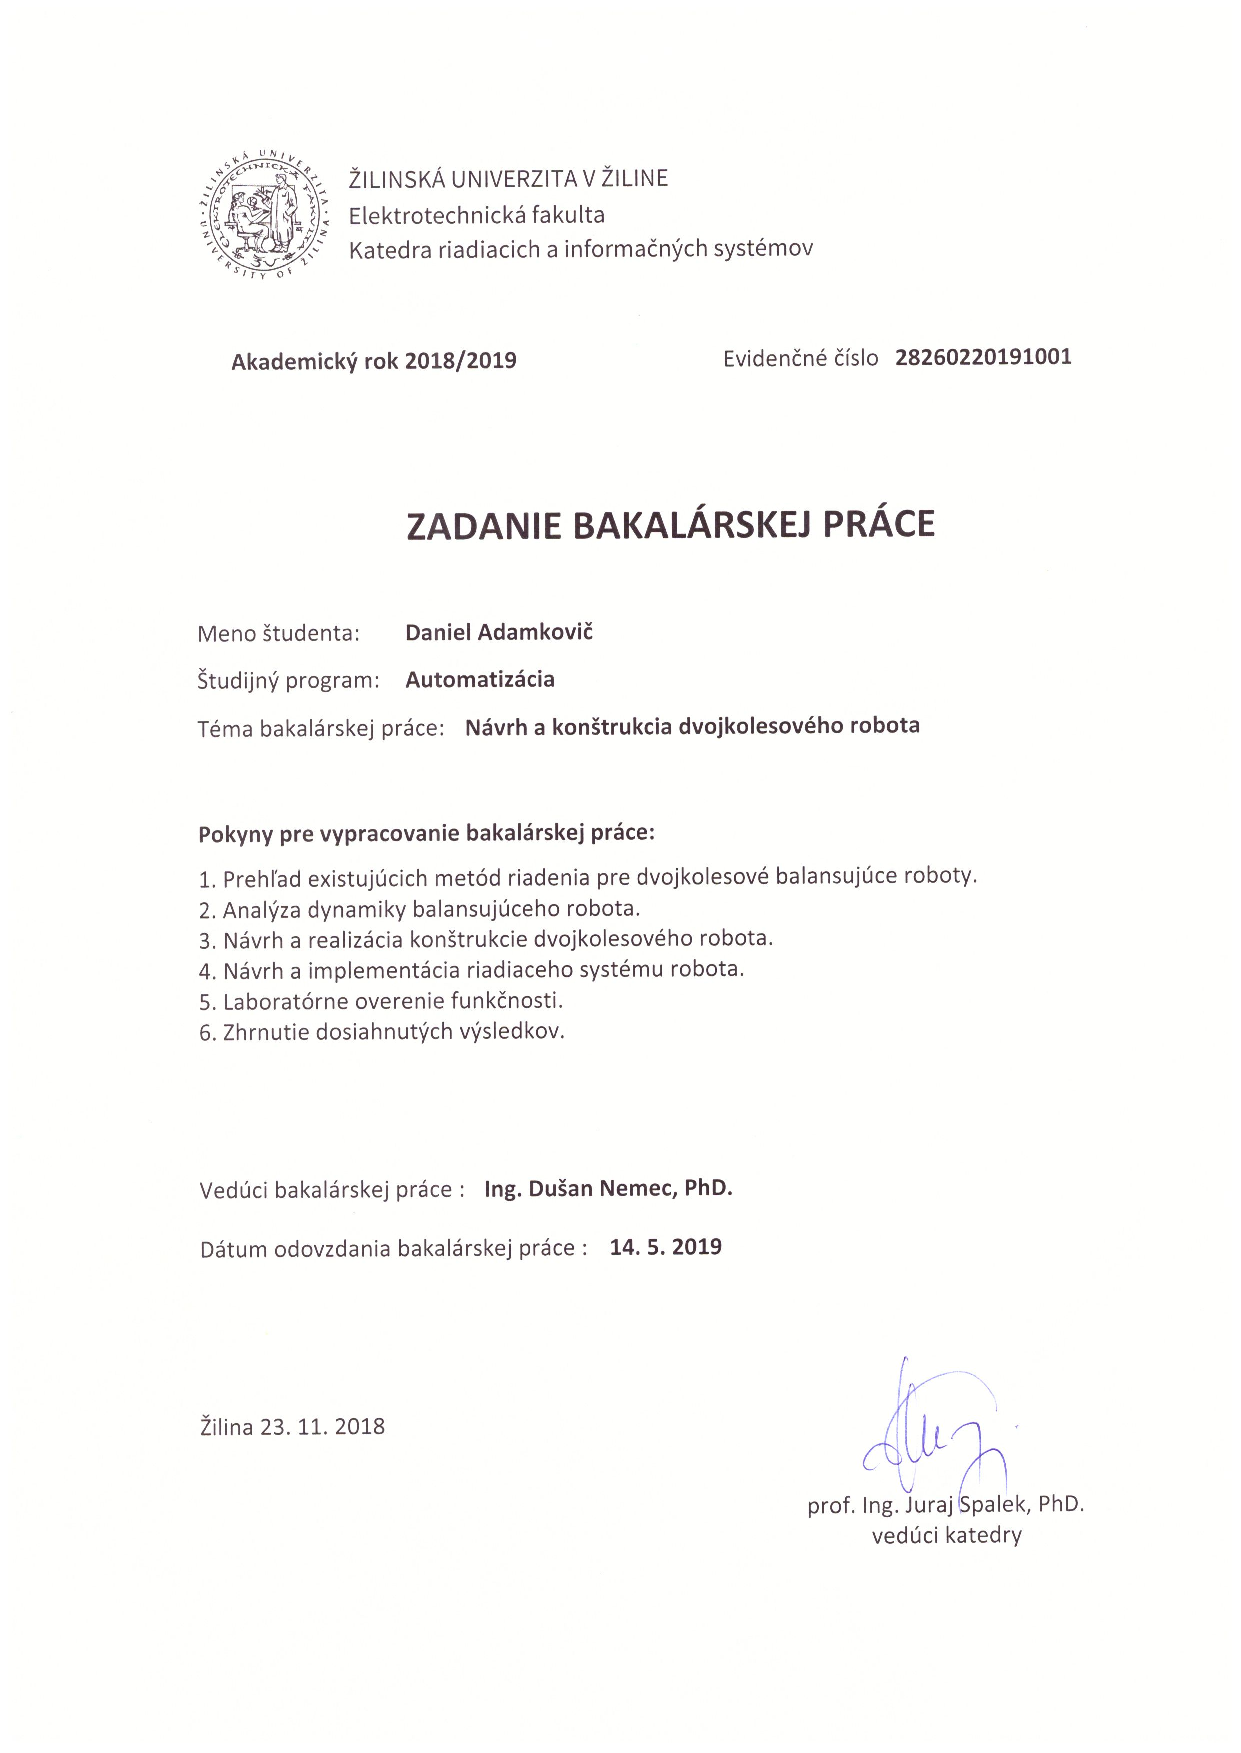
\includepdf[fitpaper]{modules/zadanie.pdf}

%-------------------------------------------------------
%				Front Matter (TOC, LOF, ...)
%-------------------------------------------------------
\frontmatter

% suppress some commands in TOC and lists
\begingroup
\renewcommand{\ac}[1]{#1}
\renewcommand{\cite}[1]{}

% Poďakovanie
\makeacknowledgements

% Abstrakt, anotácia
\makeabstract

%  TOC
\tableofcontents

% list of figures
\iftotalfigures\listoffigures\fi

% list of tables
\iftotaltables\listoftables\fi

% list of abbreviations
\acsetup{page-ref=comma,list-style=acronyms
}{
	\ifargoutempty{\printacronyms[include-classes=abbrev,heading=none]}{}{
		\unchapter{Zoznam skratiek}
		\argoutemptyFirstArg
	}
}

% dictionary
\acsetup{page-ref=none,list-style=dictstyle,extra-style=plain,extra-format={\;},only-used=false}{
\ifargoutempty{\printacronyms[include-classes=dict,heading=none]}{}{
	\unchapter{Slovník pojmov}
	\setlength{\columnseprule}{0.2pt}
	\setlength{\columnsep}{1.25cm}
	\begin{multicols}{2}
	\argoutemptyFirstArg
	\end{multicols}
}}

\endgroup % suppress some commands in TOC and lists

%-------------------------------------------------------
%						Document
%-------------------------------------------------------
\mainmatter

% !TeX spellcheck = sk_SK
\chapter{Úvod}

Dvojkolesové balansujúce roboty predstavujú v rámci robotických systémov zaujímavú skupinu robotov, ktorá účelovo predstavuje určitý medzikrok medzi klasickými, inherentne stabilnými systémami na kolesách a bipedálnymi robotmi napodobňujúcimi spôsob chôdze ľudí.
 
Avšak, kým klasické viac-kolesové roboty sa vyznačujú výbornými vlastnosťami ako v oblasti stability tak aj rýchlosti pohybu, vo všeobecnosti sú väčšie a zložitejšie (a teda aj drahšie) ako dvojkolesové roboty navrhnuté pre rovnaký účel. Výbornou ukážkou je napríklad populárny Segway, pri ktorom výrobca efektívne využil balansovanie na dvoch kolesách, bez obmedzenia užitočnosti produktu.   

Naproti tomu návrh, naprogramovanie a skonštruovanie robotických systémov s umelými nohami je v súčastnosti stále problém vyžadujúci nasdanie komplexných, ťažko naladiteľných regulátorov. Tieto systémy sa tak väčšinou javia ako príliš drahé, nespoľahlivé a pomalé na nasadenie v praxi. 

My sa v tejto práci budeme zaoberať návrhom, analýzou a konštrukciou modulárneho, balansujúceho robota, na ktorom demonštrujeme vyššie popísané vlastnosti.  
% !TeX spellcheck = sk_SK
\chapter{Prehľad existujúcich	metód riadenia pre	Dvojkolesové balansujúce roboty}

Balansujúci robot predstavuje z mechanického hľadiska inherentne nestabilnú sústavu, ktorú je pre to, aby bol takýto robot v praxi použiteľný, potrebné stabilizovať pomocou regulátora. V už existujúcich prácach sa stretávame s rôznymi druhmi implementovaných regulátorov a je teda namieste uviesť aspoň niektoré z najčastejšie používaných. V nasledujúcej časti práce sa teda budeme zaoberať  stručným popisom v praxi používaných regulátorov a uvedieme ako sme sa rozhodovali pri výbere regulátora my.

Vo všeobecnosti môžeme ako regulátor označiť každé zariadenie, ktoré v systéme zabezpečuje udržiavanie určitých fyzikálnych veličín na stanovených úrovniach. V priebehu regulácie sa pravidelne zisťuje skutočný stav objektu a porovnáva sa s požadovaným.  Regulátor následne upravuje stav systému tak, aby bol dosiahnutý požadovaný cieľ.

Jedným zo základných spôsobov rozdelenie regulátorov je na lineárne a nelineárne regulátory. Lineárne regulátory sú určené na riadenie sústav, ktorých prenosové funkcie sa vyznačujú tým, že pre ne platí princíp homogenity a superpozície. Pokiaľ chceme použiť takýto regulátor na riadenie nelineárnej sústavy, t.j. sústavy, pre ktorú neplatí princíp homogenity alebo superpozície, bude takýto regulátor pracovať korektne len ak sústava zotrvá v okolí bodu, kde je možné nájsť jej lineárnu aproximáciu. Tento proces sa nazýva linearizácia. 

Pri nelineárnych regulátoroch táto potreba linearizácie odpadá, keďže regulátory tohto typu dokážu pracovať aj s nelineárnymi sústavami. Nevýhodou práce s nelineárnymi sústavami je ale vyššia náročnosť riešenia nelineárnych diferenčných rovníc. Práve kvôli  tomuto problému existuje v praxi tendencia radšej hľadať spôsoby ako čo najpresnejšie reprezentovať nelineárne systémy lineárnymi diferenčnými rovnicami a následne použiť na ich riadenie lineárny regulátor. Je ale nutné ešte podotknúť, že reálne sa pri zohľadnení všetkých vonkajších vplyvov každá sústava javí ako nelineárna. 

Štúdiom prác, ktoré už boli napísané na tému riadenia dvojkolesového balansujúceho robota sme zistili, že medzi regulátory, ktoré sú najčastejšie pre túto úlohu používané patria lineárne regulátory:
\begin{enumerate}
\item \ac{PID} (Proportional Integral Derivative Regulator:PID)
\item \ac{LQR}  (Linear Quadratic Regulator;LQR)
\end{enumerate}

Práve týmito regulátormi sa teda budeme zaoberať v ďalšej podkapitole, no pre úplnosť ešte uvedieme, že vrámci nelineárnych regulátorov sa ako vhodné javia najmä Fuzzy PID a umelé neurónové siete.

\section{Lineárne regulátory}


V tejto časti práce zhrnieme základné poznatky o niektorých vybraných typoch lineárnych regulátoroch. Uvedieme výhodné a nevýhodné vlastnosti jednotlivých regulátorov a v závere zhodnotíme, ktorý sa pre naše potreby javí ako najvhodnejší.

\subsection{PID}


\ac{PID} regulátor je v praxi najčastejšie používaný regulátor, pričom uplatnenie nachádza  pri riadení veličín ako sú napríklad: teplota, tlak, prietok, poloha, atď. Medzi jeho výhodné vlastnosti patrí najmä robustnosť, jednoduchosť implementácie a možnosť manuálneho naladenia bez potreby použitia zložitých výpočtových techník.  Schematické znázornenie jeho zapojenia v ovládanej sústave je na \figurename~\ref{fig:PIDSchematic}

\begin{figure}
\centering
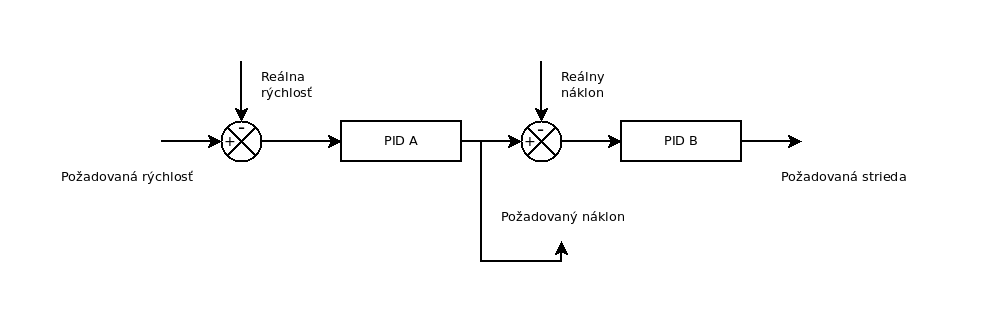
\includegraphics[width=8cm]{PIDSchematic}
\caption{Zapojenie PID}
\label{fig:PIDSchematic}
\end{figure}

Zo schémy je zrejmé, že na vstup privádzame požiadavku na výstup sústavy a od tej následne odčítavame reálne nameranú hodnotu na výstupe (spätná väzba). Takto získavame chybovú veličinu e(t), ktorá vyjadruje nakoľko sa reálna hodnota na výstupe líši od tej požadovanej. Práve s touto chybou ďalej pracuje \ac{PID} regulátor.

Samotný PID regulátor pozostáva z troch častí, ktoré mu zároveň dávajú jeho názov: proporčnej (P), integračnej (I) a derivačnej (D). Každá s týchto častí iným spôsobom reaguje na vstup do PID a proces ladenia tak pozostáva z nastavenia príslušných parametrov (opísaných nižšie) pre jednotlivé tieto časti. Kombináciou rôznych hodnôt parametrov je možné regulátor naladiť tak, aby podľa potrieb používateľa kontroloval výstupnú veličinu. 

\begin{figure}
\centering
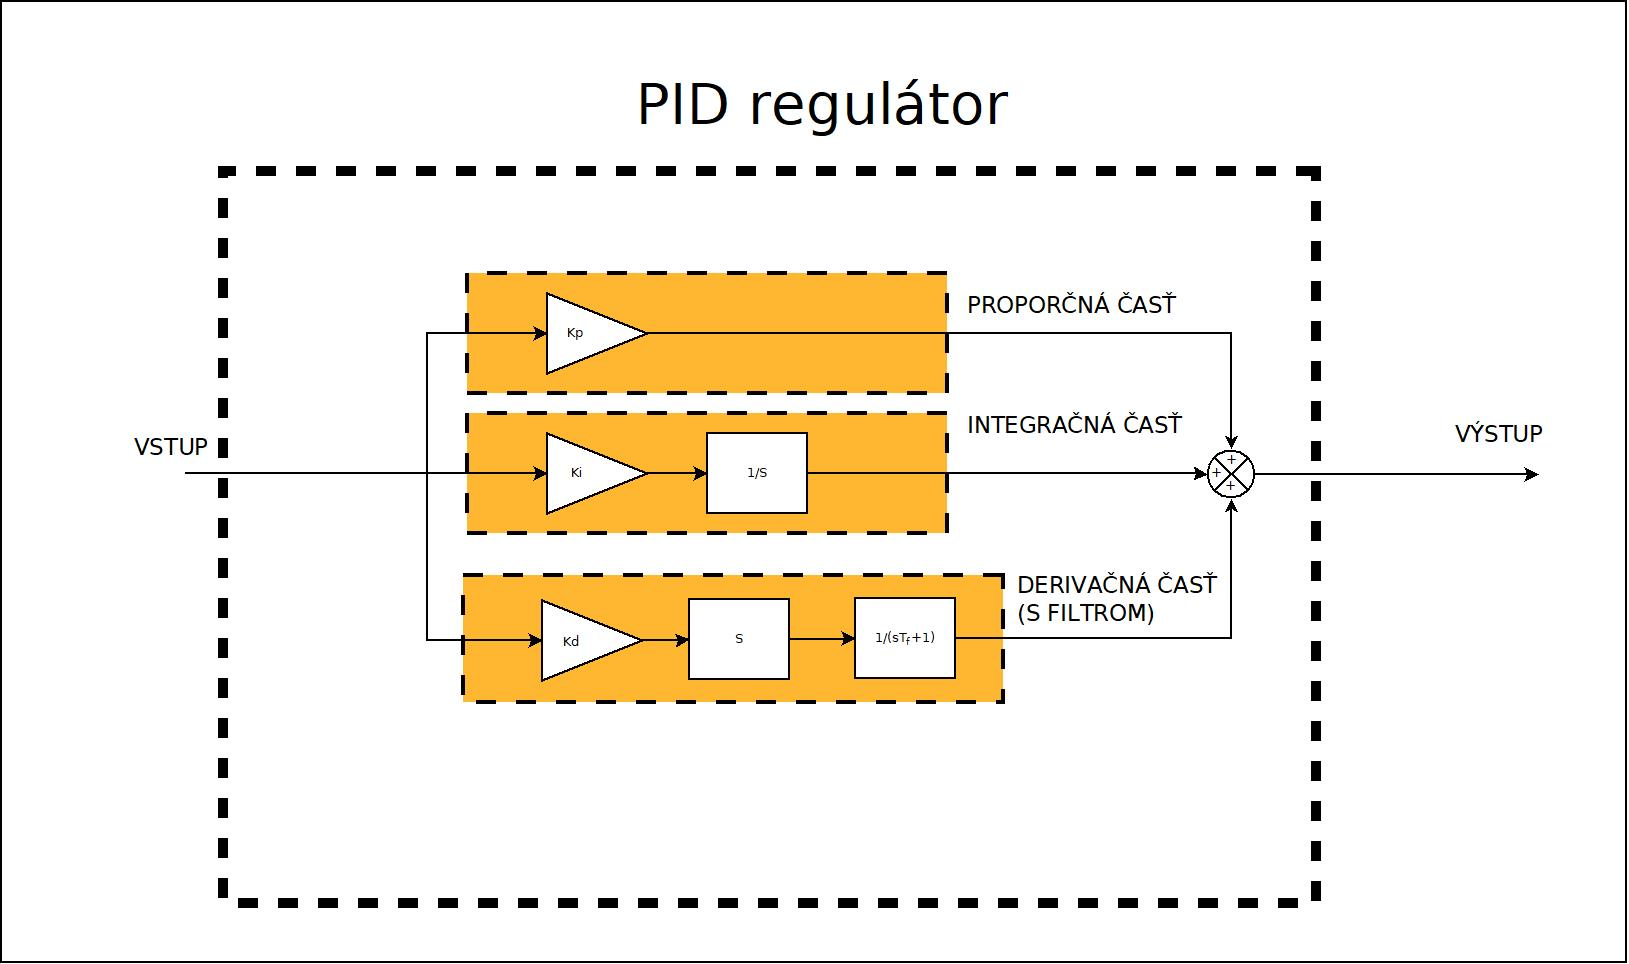
\includegraphics[width=8cm]{PIDComplete}
\caption{Štruktúra PID regulátora}
\label{fig:PIDComplete}
\end{figure}

Vychádzajúc z blokovej schémy na \figurename~\ref{fig:PIDComplete} môžeme podrobne opísať súčasti, z ktorých pozostáva \ac{PID}.

\textbf {Proporčný člen} pozostáva zo zosilňovača, ktorý má na svojom výstupe Kp násobok chyby $e(t)$ . V praxi to teda znamená, že ak je reálny výstup regulovanej sústavy voči požiadavke značne veľký $\rightarrow$ chyba je veľká a záporná, teda proporčný člen reaguje veľkým záporným výstupom. Tento následne zníži veľkosť výstupu a teda aj odchýlku od požadovanej hodnoty. Matematicky je možné vyjadriť výstup proporčného člena ako:

\begin{equation}
u_p (t)= K_p e( t )
\end{equation}

kde up(t) predstavuje výstup a e(t) chybu na vstupe člena v čase t. 

Prípadne je ešte možné použiť vyjadrenie v Laplaceovej rovine vo forme prenosovej funkcie:

\begin{equation}
\dfrac {U_p(s)} {E(s)} = K_p 
\end{equation}
kde $UP(s)$ je výstup a $E(s)$ chyba, vyjadrené v Laplaceovej rovine.

\textbf{Integračný člen} reaguje na súčet chýb, naakumulovaných od spustenia regulátora. Tento súčet je následne vynásobený konštantou $Ki$ a prenesený na výstup integračného bloku. Hlavnou výhodou integračnej časti je, že umožňuje \ac{PID} reagovať aj na veľmi malé konštantné chyby, ktoré by proporčný člen inak nebol schopný korigovať. Aj tá najmenšia chyba voči požiadavke sa totiž procesom integrovania hromadí, až kým je výstup integračného člena dostatočný na jej skorigovanie. 

Matematické vyjadrenie integračného člena je:
\begin{equation}
u_i (t)= K_i \int_0^e \! e( t ) \, \mathrm{d}t 
\end{equation}
kde $u_i(t)$ predstavuje výstup integračného člena v čase $t$. 
Prenosová funkcia je:

\begin{equation}
\dfrac{U_i(s)}{E(s)}  = K_i\dfrac{ 1}{s} 
\end{equation}
kde $U_i (s)$ je výstup vyjadrený v Laplaceovej rovine.

\textbf{Derivačný člen} v základnom zapojení pracuje so zmenou chyby za čas dt (ten sa v ideálnom prípadne limitne blíži k 0). Výhodnou vlastnosťou tohto člena teda je, že pri náhlych zmenách chyby je schopný pružne reagovať veľkou korekciou na výstupe a pri postupnom, pomalom narastaní chyby adekvátne malou korekciou. Zmenou konštanty $Kd$ vieme korigovať silu tejto reakcie na zmenu chyby.

Matematické vyjadrenie derivačného člena je:

\begin{equation}
U_d (t) = K_d\dfrac{ de(t) }{ dt }
\end{equation}
Kde $U_d(t)$ predstavuje výstup integračného člena v čase $t$.
 
Prenosová funkcia je:
\begin{equation}
\dfrac{U_d( s )}{ E(s) } = K_d s
\end{equation}
kde $U_d(s)$ je výstup vyjadrený v Laplaceovej rovine.

Existuje taktiež ale aj iná forma derivačného člena, v ktorej sa počíta so zaradením nízkofrekvenčného filtra určeného konštantou $T_f$ . Použitie tejto formy derivačného člena je obzvlášť výhodné v prípade implementácie derivačného člena na zariadení, ktoré realizuje tento člen v diskrétnej forme (mikropočítač). Pri diskrétnej forme sa totiž ako požiadavka na výstup, tak aj výstup samotný mení skokovo, čo spôsobuje pri absencií filtra silné reakcie derivačného člena, ktoré následne vyvolávajú celkovú nestabilitu  regulovaného systému.  

Filtračný člen má tvar:
\begin{equation}
F_r ( s ) = \dfrac { 1 }{ 1 + T_f s }
\end{equation}
pričom filtračnú konštantu $T_f$  spravidla určujeme podľa vzťahu:
\begin{equation}
T_f =  \dfrac {1} { 2 \pi f_c }
\label{eq:TFconst}
\end{equation}
kde $f_c$ predstavuje najvyššiu frekvenciu signálu, ktorú by ešte filter mal prepustiť. Okrem toh osa ale v praxi používa aj primitívnejšia metóda voľby $T_f$, kedy sa za $T_f$ jednoducho dosadí  celočíselný násobok konštanty $K_d$.

\textbf{Konečná forma PID} sa teda po spočítaní prenosov všetkých členov teda dá zapísať ako:
\begin{equation}
F_{PID} (s) = K_p + K_i \dfrac{1}{s} + K_d s \dfrac{ 1 } { 1 + T_f }
\label{eq:compPID}
\end{equation}

Na samotné naladenie \ac{PID} regulátora je možné použiť viacero metód, medzi inými napríklad:

\begin{itemize}
\item \textbf{Ad–hoc metóda} - veľmi primitívnou, ale pre jednoduché problémy sústavy dostačujúcou metódou je zvolenie $K_p$, $K_i$, $K_d$ parametrov náhodným dosadzovaním a pozorovaním zmien reakcií riadenej sústavy
\item \textbf{Ziegler-Nicholsová metóda} - pozostáva z vyradenia I, D zložiek a nájdenia takej hodnoty Kp, pri ktorej systém dosiahne stav na hranici stability, t.j. stavu, v ktorom sústava osciluje okolo stabilného stavu. V tomto stave odmeriame periódu oscilácií. Následným odčítaním hodnôt$K_p$, $K_i$, $K_d$ z tabuľky \ref{tab:Zieger-Nichols}, prevzatej zo skrípt\cite{SKRIPTA} získame naladený PID.
\item \textbf{Vytvorením modelu sústavy} - po nájdení matematického modelu regulovanej 	sústavy je možné vytvoriť sústavu diferenciálnych rovníc, ktoré popíšu správanie celej sústavy so zaradeným regulátorom. Tento matematický model je možné následne podrobiť analýze pomocou kritérií stability napr. Routh-	Schurovým alebo Hurwitzovým a takto nájsť  $K_p$ , $K_i$ , $K_d$, pre ktoré bude sústava stabilná. Nevýhodou tohoto postupu je ale zvýšená náročnosť procesu ladenia, ale aj nutnosť dostatočne presne poznať štruktúru sústavy na 	vytvorenie jej modelu.  
\end{itemize}

\subsection{LQR}

Pred opisom samotného princípu fungovania LQR, považujeme za potrebné uviesť čitateľa do problematiky reprezentácie systémov v tzv. stavovom priestore, nakoľko regulátor LQR pracuje práve s touto reprezentáciou systému.

Pri reprezentácií časovo invariatnej sústavy, teda sústavy, ktorej vlastnosti sa časom nemenia, v stavovom priestore pracujeme vo všeobecnosti z výrazmi tvaru:

\begin{equation}
\dot {\textbf{x}}(t) = Ax(t) + Bu(t) \linebreak
\textbf {y}(t) = Cx(t) + Dy(t)  
\end{equation}
\newpage
\begin{figure}
\centering
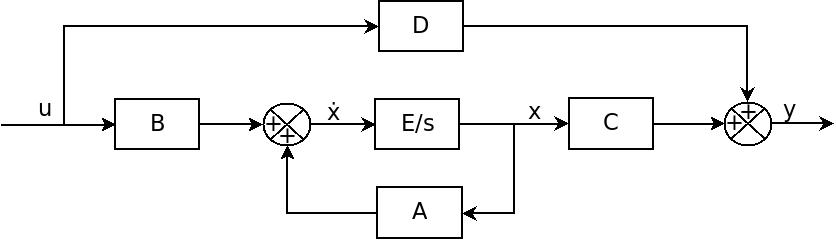
\includegraphics[width=9cm]{stavovyPriestorDiagram}
\caption{Stavový priestor - diagram}
\label{fig:stavovyPriestorDiagram}
\end{figure}

Pri takomto značení:\newline
$A$ = stavová matica systému [n x n]\newline
$B$ = vstupná matica [n x r]\newline
$C$ = výstupná matica [m x n]\newline
$D$ = matica opisujúca priamy prenos na výstup systému [m x r]\newline
$x(t)$ = stavový vektor [n x 1]\newline
$y(t)$ = výstupný vektor [m x 1]\newline
$u(t)$ = vstupný vektor [r x 1]\newline
$\dot{x}(t)$ = prvá derivácia stavového vektora [n x 1]
pričom platí, že m, n, r $\subset$ N. 

Výhody takejto reprezentácie sústav sa prejavia hlavne pri MIMO sústavách (sústavách ktoré majú viacero vstupov a výstupov). S využitím maticovej a vektorovej reprezentácie je možné aj veľmi komplexné systémy vyjadriť len pomocou týchto dvoch rovníc. Maticová reprezentácia je naviac ešte aj veľmi vhodná pre spracovanie s využitím softvérových nástrojov ako napr. Matlab.

Proces samotného vyjadrenia stavovej reprezentácie zo systému diferenciálnych rovníc je mimo rozsah tejto práce, čitateľ sa však s ním môže oboznámiť v ...

\todo[inline]{doplniť odkazy}

Po nájdení reprezentácie v stavovom priestore a overení, že daný systém je kontrolovateľný, môžeme z matice A vyjadriť póly stavovej matice sústavy. To je možné napr. výpočtom z rovnice:

\begin{equation}
\mid pE - A \mid = 0 
\end{equation}

Kde E je jednotková matica a p vektor pólov matice A.

	Pripomenieme, že pre stabilné systémy platí, že všetky reálne časti ich pólov sú záporné. Tento poznatok je možné účinne využiť v prípade nestabilných systémov a zaradiť do sústavy vhodne zvolený regulačný vektor K, ktorý nám zavedením spätnej väzby do sústavy umožní zmeniť pôvodné póly na ľubovoľné, nami zvolené, stabilné $(Re{pi}<0)$ póly. 

Reprezentácia takejto sústavy v stavovom priestore bude mať následne tvar:
\begin{equation}
u( t ) = -Kx
\label{eq:ut}
\end{equation}
\begin{equation}
\dot{\textbf{x}}(t) = Ax(t) + B(-Kx(t))
\label{eq:xDot}
\end{equation}

\begin{figure}
\centering
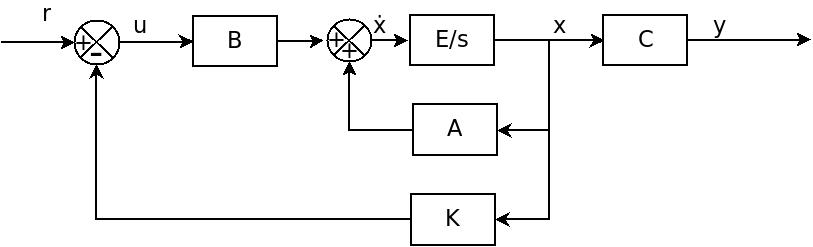
\includegraphics[width=9cm]{stavovyPriestorSV}
\caption{Stavový priestor - spätná väzba}
\label{fig:stavovyPriestorSV}
\end{figure}

Čitateľ si môže všimnúť, že na \figurename~\ref{fig:stavovyPriestorSV} už nevystupuje v schéme matica D, ktorú v danom prípade uvažujeme ako nulovú – veličina na vstupe nie je teda privádzaná priamo na výstup. Členom r v schéme na \figurename~\ref{fig:stavovyPriestorSV} rozumieme referenciu, ktorej zmenou vieme upraviť požiadavku na výstup systému.

Vyššie sme spomínali, že vektor K je možné zvoliť tak aby boli dosiahnuté požadované póly, problémom ale je určiť aké póly sú pre danú sústavu ideálne. Pri zvolení príliš negatívnych pólov bude regulátor natoľko agresívny, že ho nebude možné v praxi realizovať a naopak, pokiaľ nebudú póly dostatočne záporné, bude regulácia trvať pridlho na to aby bola praktická.  Práve tu prichádza ako riešenie do úvahy regulátor LQR, ktorý je využitím kvadratickej „cenovej“ funkcie schopný prideliť každej sledovanej veličine na výstupe „váhu“. Táto váha určí nakoľko budú pre regulátor dôležité zmeny jednotlivých veličín. LQR následne zvolí K také, aby regulátor pracoval podľa požiadaviek.

Ako vyplýva z názvu regulátora, pre svoju činnosť využíva princíp minimalizácie cenovej funkcie J, ktorá je pre spojitý a konečný časový úsek definovaná ako:

\begin{equation}
J = \dfrac {1} {2} x^T (T)P_1 x(T)  + \dfrac {1} {2} \int_0^T \! ( x^T Qx + u^T Ru) \, \mathrm{d}t 
\label{eq:cenovaFunkcia}
\end{equation}

kde $Q \geq 0$; $R > 0$; $P1 \geq 0$ sú symetrické, kladné matice. $Q$,$ R$ predstavujú váhy, ktoré sú priradené sledovaným veličinám.
Riešením rovnice \figurename~\ref{eq:cenovaFunkcia} je $P(t)$, nájdené vyriešením tzv. aritmetickej Riccatiho rovnice :

\begin{equation}
- \dot {P} = PA + A^T P - PBR^{-1} B^T P + Q;	\newline
P( T ) = P_1
\label{eq:riccatiEq}
\end{equation}

Následkom rovnice \figurename~\ref{eq:riccatiEq} je po spätnom chode a vyriešení pre $K$ možné vyjadriť $u(t)$ z rovnice \figurename~\ref{eq:ut} ako:
\begin{equation}
u( t ) = -R^{-1} B^T P( t )x
\end{equation}

Keďže riešenie týchto rovníc je do značnej miery komplikované a jednoznačne mimo rozsah tejto práce uvedieme len, že pri použití nastroja Matlab je možné nájsť K veľmi jednoducho a to použitím funkcie: K = lqr(A, B, Q, R).

Pred implementáciou LQR je ale ešte potrebné adresovať otázku voľby R, Q matíc. Predpokladajme matematický model balansujúceho robota v stavovom priestore vyjadrený dosadením do rovnice \figurename~\ref{eq:xDot} ako:
\begin{equation}
\dot {\textbf {x}} = (A - BK) \begin{bmatrix}
d \\
\dot{d} \\
\theta \\
\dot{\theta} 
\end{bmatrix}
\end{equation}
kde: 

\quad $d$ = poloha základne robota 

\quad $\dot{d}$ rýchlosť  základne robota 

\quad $\theta$ = uhol natočenia šasi robota 

\quad $\dot{\theta}$ = uhlová rýchlosť robota

Ďalej uvažujeme Q také, že:
\begin{equation}
Q = \begin{bmatrix}
w_1 & 0 & 0 & 0 \\
0 & w_2 & 0 & 0 \\
0 & 0 & w_3 & 0 \\
0 & 0 & 0 & w_4
\end{bmatrix}
\end{equation}
\newline
Predpokladajme, že maximálne dovolené odchýlky od požadovanej hodnoty sú:
\begin{itemize}
\item $0,005 m $pre polohu základne → $w_1$ = $(0,005)^{-2}$
\item $0,0005 m.s^-1$ pre rýchlosť základne → $w_2$ = $(0,0005)^{-2}$
\item $0,02 rad$ pre uhlovú odchýlku šasi → $w_3$ = $(0,02)^{-2}$
\item $0,0001 rad.s^{-1}$ pre uhlovú rýchlosť šasi → $w_4$ = $(0,0001)^{-2}$
\end{itemize}

Po určení Q by sme podobným spôsobom postupovali aj pre R až kým by sme našli hodnoty, ktoré pre sústavu fungujú uspokojivo. 

\section{Zhrnutie a výber regulátora}
Medzi značné výhody PID regulátora patrí jeho jednoduchá implementácia a nízka náročnosť na výpočtový výkon realizačného hardvéru. Ladenie je možné ako exaktnými, matematickými metódami tak aj metódami založenými na empiricky zozbieraných dátach. Nevýhodou PID je ale,  že jeho využitie je obmedzené na SISO systémy, t.j. systémy s jednou vstupnou a jednou výstupnou veličinou – čo napríklad v našom prípade nezaručí stabilizáciu polohy aj riadenie robota súčastne. Tento nedostatok je ale možné prekonať použitím viacerých vhodne kombinovaných PID regulátorov, čo však zvyšuje náročnosť ich správneho naladenia.

Hlavnou výhodou využitia LQR na reguláciu sústavy je, možnosť riadiť jediným regulátorom všetky nami sledované výstupné veličiny, čim je možné dosiahnuť veľmi komplexné riadenie robota. Pri návrhu regulátora je taktiež možné zvoliť, ktoré sledované veličiny sú pre nás najdôležitejšie. Cenou za takúto presnosť riadenia je ale výrazne vyššia náročnosť výpočtov pri ladení regulátora ako aj nutnosť pracovať s matematickým modelom sústavy. Komplikovanejšie výpočty taktiež spôsobia, že v porovnaní s PID bude dĺžka trvania riadiacej slučky pri použití totožného hárdveru dlhšia čo môže viesť k zhoršeniu vlastností robota.

Po zohľadnení vlastností oboch regulátorov sme sa rozhodli pre použitie PID regulátora. Napriek niektorým jeho nevýhodným vlastnostiam bola jednoduchosť jeho implementácie rozhodujúcim faktorom pri našej voľbe. Viacero prác už demonštrovalo uspokojivé výsledky pri použití PID na riadenie balansujúceho robota a teda vieme, že ide o regulátor dostačujúci na naše účely a na rozdiel od LQR má autor s jeho používaním predošlé skúsenosti. 

Kvôli neschopnosti PID riadiť viacero výstupov zároveň budeme pri našej realizácií pracovať s viacerými PID regulátormi zaradenými do kaskády. V takomto zapojení sa zvyčajne uvažuje používa rozdielna dĺžka riadiacich slučiek - teda  rozdielne dt pre jednotlivé PID. Viac sa danou problematikou budeme zaoberať priamo v kapitole venovanej našej implementácií regulátora.
% !TeX spellcheck = sk_SK
\chapter{Analýza dynamiky balansujúceho robota}
\label{ch:analyza}

Dvojkolesový robot predstavuje z mechanického uhla pohľadu sústavu podobnú prevrátenému kyvadlu – teda sústavu, ktorá je inherentne nestabilná a vyžaduje teda implementáciu robustného regulátora. Aby bol tento návrh možný potrebujeme vytvoriť matematický model tohto systému, ktorý nám umožní navrhúť optimálny regulátor. Po zvážení sme usúdili, že bude výhodné takýto model vytvoriť ako pre časť podvozku s kolesami tak aj pre šasi robota, ktoré tvorí prevrátené kyvadlo a tieto následne skombinovať.
Pracovať budeme s modelom navrhnutým Rich Chi Ooi \cite{Oochi2003} a mierne upraveným v práci\cite{TWIP}.

\section{Model kolesa}

Matematický model správania sa kolesa nebudeme odvádzať pre každé koleso zvlášť, ale budeme predpokladať, že obe kolesá sú identické a teda aj rovnice budú pre obe rovnaké.
\begin{figure}
\centering
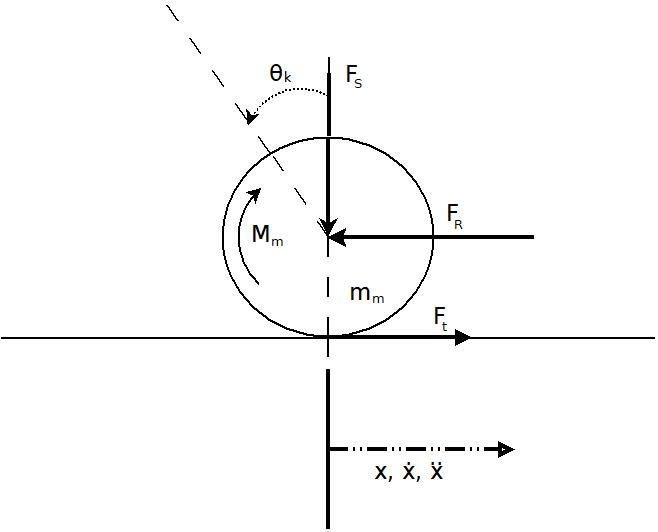
\includegraphics[width=8cm]{wheelForces}
\caption{Model kolesa}
\label{fig:wheelForces}
\end{figure}

\figurename~\ref{fig:wheelForces} znázorňuje koleso robota aj so všetkými silami, ktoré naň pôsobia, pričom:

\begin{multicols}{2}
\begin{itemize}
\item $\theta$ = uhol náklonu šasi
\item $m_k$ = hmotnosť kolesa 
\item $F_s$ = sila, ktorou na kolesa pôsobí šasi
\item $F_R$ = reakčná sila medzi kolesom a šasi
\item $F_t$ = trecia sila medzi zemou a kolesom
\item $J_k$ = zotrvačnosť kolesa
\item $r$ = polomer kolesa 
\item $M_m$ = točivý moment
\item $x$ = poloha v x-ovej osi
\end{itemize}
\end{multicols}

V rovniciach budeme ďalej predpokladať, že robot sa nepohybuje do strán ale len vpred alebo vzad. Do úvahy budeme musieť ale vziať to, že robot bude pri pohybe ovplyvňovaný ako vonkajšími stimulmi tak aj samotným momentom motora. Na začiatok využitím Newtonovho zákona pohybu v X-ovej osi odvodíme:
\begin{equation}
\begin{gathered}
\sum{F_x} = ma \\
m_k \ddot{x} = F_t - F_R
\end{gathered}
\label{eq:forceOnWheeles}
\end{equation}
A potom vyjadríme súčet momentov okolo stredu kolesa:
\begin{equation}
\begin{gathered}
\sum{M} = J \alpha \\
J_k\ddot{\theta} = M - F_f r
\end{gathered}
\label{eq:zotrvacnost}
\end{equation}

Ak teda vyjadríme točivý moment DC motora ako rozdiel zotrvačnosti motora vynásobeného okamžitým uhlovým zrýchlením a momentu záťaže môžeme pokračovať v odvodzovaní:
\begin{equation}
\begin{gathered}
M_m = J \dfrac{d \mathrm{\omega}}{d \mathrm{t}} - M_Z
\\
M = M_m - M_Z = \dfrac{-K_M K_e}{R} \dot{\theta}+ \dfrac{K_M}{R} V_m
\end{gathered}
\label{eq:moment}
\end{equation}

kde:
$\quad K_Z$ = moment záťaže

$\quad K_M$ = momentová konštanta

$\quad K_e$ = elektrická konštanta motora

$\quad R$ = odpor vinutia motora

$\quad U_m$ = el. napätie na motore

Konštanty $K_M$, $K_e$ je možné získať zo vzťahov \eqref{eq:motoroveKonstanty}:
\begin{equation}
K_e = \dfrac{V_X}{\omega} \quad \quad K_M = \dfrac{F_X r}{I_X}
\label{eq:motoroveKonstanty}
\end{equation}


Dosadením do \eqref{eq:zotrvacnost} z \eqref{eq:moment} tak získame:
\begin{equation}
F_f = \dfrac{-K_M K_e}{Rr}\dot{\theta}_k + \dfrac{K_M}{Rr}U_m - \dfrac{K_k}{r}\ddot{\theta}_k
\end{equation}
Túto rovnicu je možné prepísať pomocoou \eqref{eq:forceOnWheeles} a nájsť tak rovnicu pre jedno koleso:
\begin{equation}
\begin{gathered}
m_m \ddot{x} = F_f - F_R =  \dfrac{-K_m K_e}{Rr}\dot{\theta}_k + \dfrac{K_M}{Rr}U_m - \dfrac{J_k}{r}\ddot{\theta}_k - F_R \\
\downdownarrows
\\
\theta = \dfrac{x}{r}
\\
\downdownarrows
\\
m_m \ddot{x} = F_f - F_R = \dfrac{-K_M K_e}{R r^2}\dot{x}_k + \dfrac{K_M}{Rr}U_m - \dfrac{J_k}{r^2}\ddot{x}_k - F_R
\end{gathered}
\end{equation}

Vynásobením dvoma (dve kolesá) získavame kompletný model podvozku:
\begin{equation}
\begin{gathered}
2m_m \ddot{x} = 2F_f - 2F_R = \dfrac{-2K_M K_e}{R r^2}\dot{x}_k + \dfrac{2K_M}{Rr}U_m - \dfrac{2J_k}{r^2}\ddot{x}_k - 2F_R
\\
2(m_m - \dfrac{2J_k}{r^2}) \ddot{x} = \dfrac{-2K_M K_e}{R r^2}\dot{x}_k + \dfrac{2K_M}{Rr}U_m - 2F_R
\end{gathered}
\label{eq:wheels}
\end{equation}

\section{Model šasi}


\begin{figure}[b]
\centering
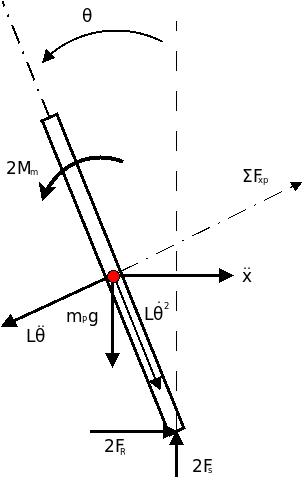
\includegraphics[width=4cm]{chasisPend}
\caption{Model šasi}
\label{fig:chasisPend}
\end{figure}

Na \figurename~\ref{fig:chasisPend} sú znázornrné sily pôsobiace na šasi robota pri pohybe, pričom:

$\quad L$ = dĺžka šasi, meraná od stredu kolies

$\quad m_p$ = hmotnosť šasi

$\quad \theta$ = uhol náklonu šasi

$\quad \sum{F_{xp}}$ = súčet síl na virtuálnej osi xp

Význam ostatných veličín je zhodný s definíciami v predchádzajúcej časti. Je teda zjavné, že podľa očakávaní sú sily pôsobiace na podvozok premietnuté aj do modelu šasi. Z Newtonovho zákona po úprave dostaneme rovnicu v tvare:
\begin{equation}
2F_R = m_p \ddot{x} + m_p L \ddot{\theta} cos{\theta} - m_p L\dot{\theta}^2 sin\theta
\label{eq:horizontal}
\end{equation}

Táto rovnica predstavuje súčet síl na horizonálnej osi. Pre sily pôsobiace ne virtuálnej osi $F_px$, kolmo na šasi, platí vzťah \eqref{eq:perpend} a súčet momentov síl okolo ťažiska šasi je vyjadrený v \eqref{eq:around_center}.
\begin{equation}
2F_R cos\theta + 2F_S sin\theta - m_p g sin\theta - m_p L \ddot{\theta} = m_p \ddot{x}cos\theta
\label{eq:perpend}
\end{equation}
\begin{equation}
-2F_R L cos\theta - 2F_S L sin\theta - 2M_m = J_p \ddot{\theta}
\label{eq:around_center}
\end{equation}

Točivý moment motorov je potrebné linearizovať a teda:
\begin{equation}
2M_m = \dfrac{-2K_M K_e \dot{x}}{Rr} + \dfrac{2K_M U_m}{R}
\label{eq:linear_moment}
\end{equation}

Po dosadení \eqref{eq:linear_moment} do \eqref{eq:around_center} dostaneme \eqref{eq:subst}. Následne upravíme \eqref{eq:perpend} vynásobením $-L$ a prepísaním do tvaru \eqref{eq:rearanged}:
\begin{equation}
-2F_R L cos\theta - 2F_S L sin\theta = \dfrac{-2K_M K_e \dot{x}}{Rr} + \dfrac{2K_M U_m}{R} + J_p\ddot{\theta}
\label{eq:subst}
\end{equation}
\begin{equation}
-2F_R L cos\theta - 2F_S L sin\theta = -m_p g L sin\theta - m_p L^2 \ddot{\theta} - m_p L \ddot{x} cos\theta
\label{eq:rearanged}
\end{equation}

Odčítaním týchto dvoch rovníc dostávame:
\begin{equation}
\dfrac{-2K_M K_e \dot{x}}{Rr} + \dfrac{2K_M U_m}{R} + J_p\ddot{\theta} = -m_p g L sin\theta - m_p L^2\ddot{\theta} - m_p L \ddot{x} cos\theta
\label{eq:chasis}
\end{equation}

Z rovnice \eqref{eq:wheels} môžeme odstrániť člen $2F_R$ nahradením z \eqref{eq:horizontal}:
\begin{equation}
2(m_m - \dfrac{2J_k}{r^2}) \ddot{x} = \dfrac{-2K_M K_e}{R r^2}\dot{x}_k + \dfrac{2K_M}{Rr}U_m - m_p \ddot{x} - m_p L \ddot{\theta} cos\theta - m_p L \ddot{\theta}^2 sin\theta
\label{eq:wheels}
\end{equation}

Po vyjadrení \eqref{eq:chasis} a \eqref{eq:wheels} je potrebné rovnice linearizovať. Pri linearizácií predpokladaáme, že uhol $\theta = 0 + \varphi$, kde $\varphi$ predstavuje malý uhol náklonu robota. Výsledkom linearizácie a následnej úpravy rovníc je výsledný model balansujúceho robota:
\begin{equation}
\begin{gathered}
\ddot{\varphi} = \dfrac{m_p L}{J_P L^2}\ddot{x} + \dfrac{2K_M K_e}{Rr(J_P + m_p L^2)}\dot{x} - \dfrac{2K_M}{R(J_P + m_p L^2)} U_m + \dfrac{m_p g L}{(J_P + m_p L^2)}\varphi
\\
\\
\ddot{x} = \dfrac{2K_M}{Rr(2m_k - \dfrac{2J_k}{r^2} + m_p)} U_m - \dfrac{2K_M K_e}{Rr^2(2m_k - \dfrac{2J_k}{r^2} + m_p) }\dot{x} + \dfrac{m_p L}{2m_k - \dfrac{2J_k}{r^2} + m_p}\ddot{\varphi}
\end{gathered}
\end{equation}
\chapter{Návrh a realizácia konštrukcie dvojkolesového robota}

Proces návrhu hardvérového riešenia robota sme začali vytvorením zoznamu komponentov, potrebných pre realizáciu robota. Pri výbere komponentov a celkovom návrhu robota sme brali do úvahy požiadavku na modulárnosť robota. Pod pojmom modulárnosť rozumieme skonštruovanie robota tak, aby jednotlivé jeho časti mohli byť v prípade potreby jednoducho vymenené alebo upravené bez potreby väčších zásahov do celkovej konštrukcie. 

Robota sme teda rozdelili do viacerých funkčných celkov a pre každý z týchto celkov sme vytvorili samostatný zoznam komponentov. Vďaka tomuto postupu sme nielen znížili možnosť výberu nevyhovujúcich súčiastok, ale aj zabezpečili, že naše riešenie bude v prípade potreby škálovateľné a jednotlivé celky bude ľahké pozmeniť alebo doplniť o dodatočné časti. 


\underline{\textbf{Funkčné celky balansujúceho robota:}}
\begin{itemize}
\item napájanie
\item pohon
\item komunikácia
\item senzory
\item riadiaci mikropočítač
\end{itemize}

\section{Zoznam použitých komponentov}

V nasledujúcej časti práce opíšeme nami vybrané komponenty, ktoré boli využité pri konštrukcii robota. Zameriame sa hlavne na dôvod voľby daného komponentu, porovnáme špecifikácie použitých komponentov s našimi požiadavkami a zhodnotíme, ako dobre sa komponent hodí pre naše použitie.


\subsection{Napájanie}
Táto podkapitola obsahuje komponenty, ktoré poskytujú vhodné napájanie ostatným častiam robota.
\subsubsection{Batéria}
Pri výbere batérie sme sa snažili nájsť nabíjateľný model, ktorý by nám poskytol pri nízkej hmotnosti čo najvyššiu kapacitu, relatívne vysoký maximálny výstupný prúd a  výstupné napätie pohybujúce sa v rozmedzí 6 V až 12 V, ktoré je dostatočné pre väčšinu bežne dostupných jednosmerných motorov. Rozhodli sme sa pre 12V lítium-iónovú (Li-ion) batériu, využívajúcu tri 3,7 V články typu 18650. Kapacita batérie je 3300 mAh, maximálny okamžitý odoberaný prúd 5 A a maximálny pracovný prúd 3A. K nej priložený nabíjací adaptér je schopný dobíjať ju prúdom 1 A pri 12,6 V. Spolu s relatívne nízkou hmotnosťou 150g sa teda batéria z \figurename~\ref{fig:bateria} po každej stránke javí ako dobrá voľba. 

\begin{figure}[h]
\centering
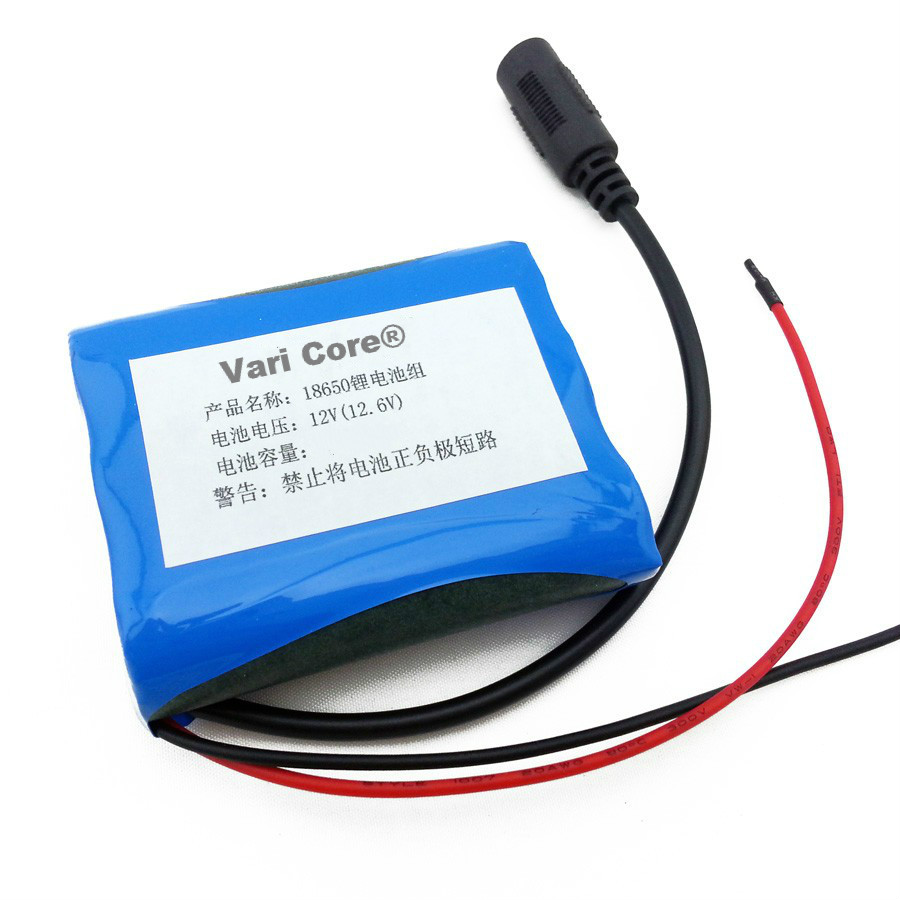
\includegraphics[width = 6cm]{bateria}
\caption{Li-ion batéria\cite{VariCore}}
\label{fig:bateria}
\end{figure}


\bgroup
\def\arraystretch{1.8}
\begin{table}[h]
\centering
\begin{tabular}{|c|c|c|c|c|}
\hline
Výs. napätie [V] & Max. výs. prúd [A] & Pracovný prúd [A]  & Hmotnosť [kg]&Technológia\\
\hline
 12& 5 & 3  & 0.15& Li-ion \\
\hline
\end{tabular}
\caption{Parametre batérie}
\label{tab:bateria}
\end{table}
\egroup

\subsubsection{Napäťový regulátor pre logické obvody}
Jedným z možných riešení pre napájanie logických obvodov robota, bolo použitie sekundárnej $5~V$ batérie. Toto riešenie sa ale nejavilo v tomto prípade ako optimálne, keďže druhá batéria by zaberala miesto a vyžadovala si samostatný napájací adaptér. Rozhodli sme sa preto využiť už zabudovanú $12~V$ batériu napájajúcu motory v kombinácii s paralelne pripojeným napäťovým regulátorom. 

Rozhodovali sme sa medzi rozšíreným integrovaným obvodom L7805CV, ktorý predstavuje $5~V$ lineárny napäťový regulátor a modulom MP1584. Modul MP1584\figurename~\ref{fig:napRegulator} je spínaným napäťovým regulátorom a obsahuje integrovaný obvod LM2596\cite{LM2596} . Vďaka vlastnostiam LM2596, medzi ktoré patrí vysoká účinnosť (až 92\%), malé kolísanie výstupného napätia a možnosť riadenia výstupného napätia od $4~V$ – $35~V$ sme sa nakoniec rozhodli použiť ako napäťový regulátor modul MP1584.

\begin{figure}[h!]
\centering
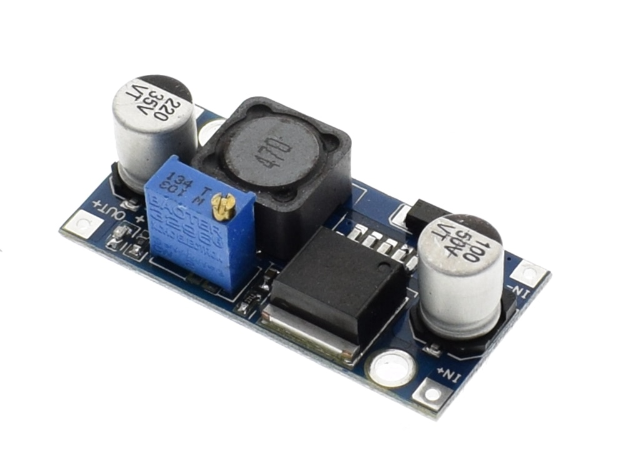
\includegraphics[width=6cm]{napRegulator}
\caption{Modul MP1584\cite{MP1584}}
\label{fig:napRegulator}
\end{figure}

\subsection{Pohon}
Pre samotný pohyb robota je potrebné správne zvoliť vhodný typ motora a obvodu, ktorý bude môcť podľa pokynov mikropočítača dané motory ovládať. V našom prípade sme vyberali motory, ktoré budú poháňať kolesá robota, aj servomotor umožňujúci robotu pohybovať sa aj po naklonených plošinách.

\subsubsection{Motory}
V prípade motorov sme mali na výber z viacerých možností, pričom hlavným kritériom bolo, že sa musí ísť o jednosmerné motory primeranej veľkosti. Aj tak sme ale mohli voliť medzi bezkomutátorovým, krokovým a motorom s permanentnými magnetmi. Po úvahe a prieskume bežne dostupných motorov sme sa rozhodli pre klasický motor s permanentnými magnetmi využívajúci komutátor. Tento motor má niekoľko nevýhod, ako sú napríklad malá presnosť v porovnaní s krokovým motorom a menší moment spolu s rýchlejším opotrebením v porovnaní s motorom bez komutátora. Napriek týmto nevýhodám sú tieto motory ale vhodné pre naše účely, lebo sú lacné, jednoduché na ovládanie a dostupné v mnohých konfiguráciách. 

Po zvážení sme sa rozhodli pre $12~V$ motory typu GM25-370CA, s integrovanou prevodovkou 1:21 a zabudovanými dvojkanálovými enkodérmi, ktoré nám umožnia odometrickým meraním sledovať zmenu pozície kolies napojených na motor. Dokumentácia uvádza max. rýchlosť nezaťaženého motora ako 280 \ac{RPM} (otáčok za minútu), pričom túto max. rýchlosť potvrdili aj naše merania. Výhodou týchto motorov je aj to, že je ich možné dostať v konfigurácii priamo určenej pre robotické platformy podobné našej spolu s kolesami a kovovým podvozkom. Nevýhodou týchto motorov je relatívne veľká vôľa kolies a nízke rozlíšenie integrovaných enkodérov.  

\begin{figure}[h!]
\centering
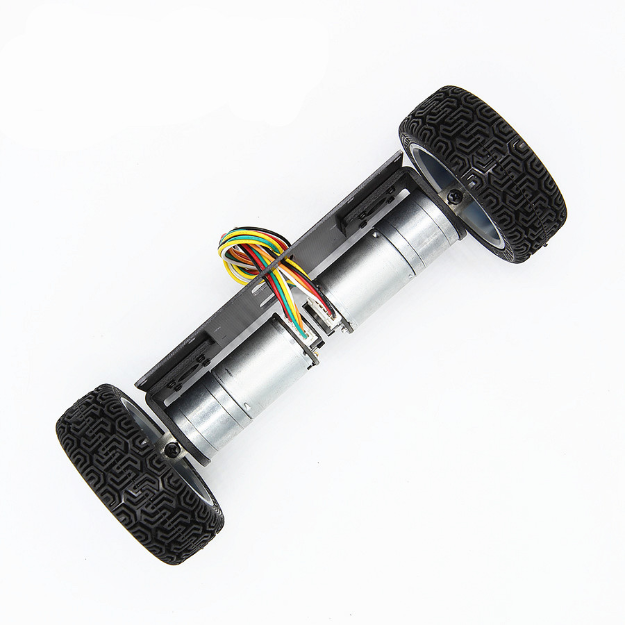
\includegraphics[width=6cm]{motorPlatforma}
\caption{Platforma s motormi\cite{wheelBase}}
\label{fig:motorPlatforma}
\end{figure}

\subsubsection{H-mostík}
Keďže mikropočítač nie je bez externej elektroniky schopný sám dodávať do motora potrebný výkon, je potrebné spolu s ním použiť tzv. H-mostík. Ten predstavuje principiálne iba štyri elektricky ovládané spínače \figurename~\ref{fig:h_bridge_scheme}, ktoré podľa svojej konfigurácie menia smer toku prúdu motorom - teda smer otáčania motora. Naše požiadavky na H-mostík boli: vysoká účinnosť, jednoduché prepojenie s mikropočítačom, galvanicky oddelené vstupy mikropočítača a schopnosť dodať motorom dostatočný výkon (výrobca uvádza maximálny odber $3,5~A$ na motor). 

Našou voľbou bol dvojitý H-mostík kompatibilný s integrovaným obvodom L298, ktorý spĺňa všetky naše požiadavky a je schopný dlhodobo dodávať do motorov až $7~A$ pri napätí $12~V$. Tento obvod je možné prepojiť s mikropočítačom pomocou šiestich vstupov, pričom štyri slúžia na výber konfigurácie spínačov a dva prijímajú \ac{PWM} signál, ovládajúci pripojenie batérie na vstup motorov. Je teda možné jednoducho meniť striedu jednotlivých motorov a tým aj ich rýchlosť. Pre svoju správnu činnosť vyžaduje tento H-mostík napájanie $5~V$, to nám poskytne nami použitý napäťový regulátor. 

\begin{figure}
\centering
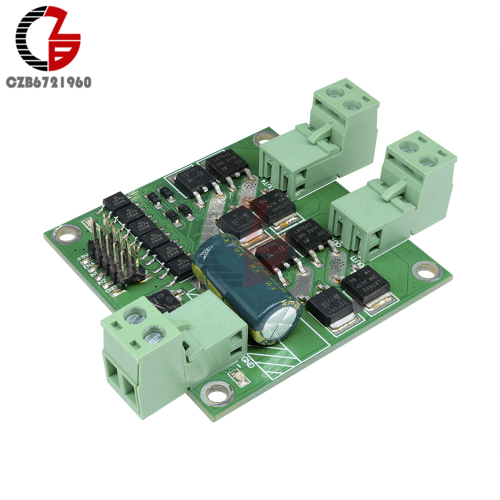
\includegraphics[width=6cm]{hMostik}
\caption{H-mostík komaptibilný s L298\cite{hBridge}}
\label{fig:hMostik}
\end{figure}

\subsubsection{Servomotor}
Jednou z dodatočných požiadaviek na náš balansujúci robot bolo, aby sa šasi robota mohlo pohybovať do strán nezávisle od platformy s kolesami. Táto funkcionalita nám v praxi poskytne vyššiu kontrolu nad robotom v zákrutách, na naklonených plošinách a do určitej miery zníži pravdepodobnosť pádu v prípade pôsobenia silou na bočnú časť robota.

Za optimálne riešenie sme považovali jednoduché servo HJ S3315D určené prevažne na modelárske účely. Toto servo dodatočne taktiež spojí platformu s kolesami a šasi robota, ktorým bude takto možné v prípade potreby hýbať o presne určené uhly. V takejto konfigurácii  obmedzenie pohybu serva v rozmedzí -90º až 90º nepredstavuje problém.


\begin{figure}[h]
\centering
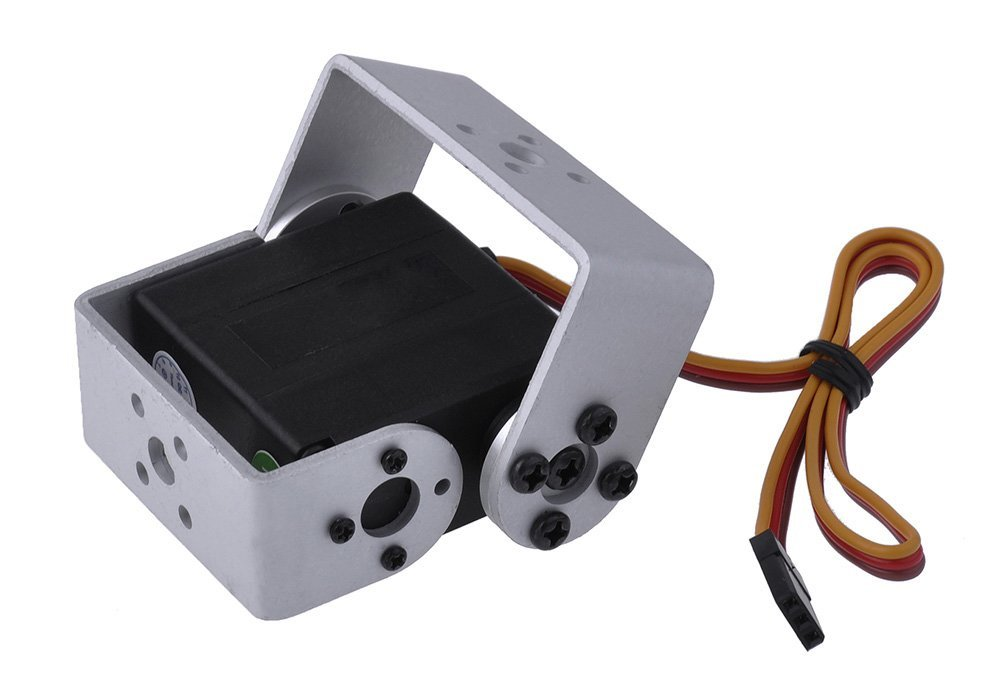
\includegraphics[width=8cm]{servoMotor}
\caption{Servo motor HJ S3315D\cite{servoMotor}}
\label{fig:servoMotor}
\end{figure}
\subsection{Komunikácia - Bluetooth modul}
Okrem neriadeného balansovania na mieste musí byť robot tiež schopný prijímať od operátora na diaľku príkazy a pohybovať sa v priestore podľa pokynov. Taktiež je nutné, aby bol robot v prípade požiadania operátora schopný poskytnúť základné informácie o svojom stave, napr. úroveň nabitia batérie, priemernú rýchlosť pohybu za určitý časový interval, okamžitý uhol náklonu,… Tieto informácie musí byť robot schopný poskytnúť s čo najmenším oneskorením, bezdrôtovo a minimálne na vzdialenosť 10 metrov.  
\begin{figure}[h!]
\centering
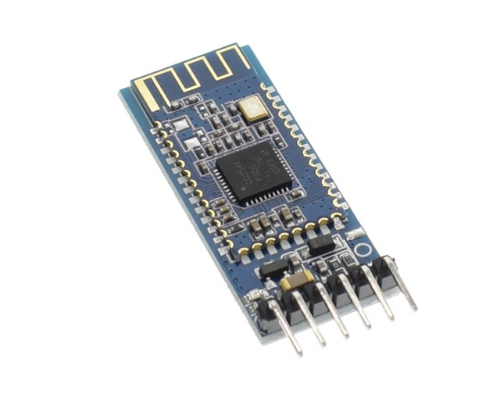
\includegraphics[width=8cm]{bluetoothModul}
\caption{HC05-Bluetooth modul\cite{bluetoothModule}}
\label{fig:bluetoothModul}
\end{figure}
Rozhodli sme sa použiť Bluetooth vysielač/prijímač HC-05. Tento modul sa vyznačuje integrovanou anténou, nízkym operačným napätím (min. $1.3~V$) a je schopný prijímať aj odosielať dáta pomocou štandardného rozhrania \ac{UART} (Universal Asynchronous Reciever-Transmitter). Dosah tohto modulu je na stránke predajcu uvádzaný až do $10~m$.

Využitím tohoto modulu v robotovi aj v ovládači, ktorým ho budeme ovládať zabezpečíme možnosť odosielať jednoduché povely na riadenie robota aj prijímať komplexné dáta o jeho aktuálnom stave.

\subsection{Senzory}
Pod senzormi rozumieme všetky časti robota, ktoré mu umožňujú získavať informácie o jeho okolitom prostredí, ale aj o jeho vlastnom stave. Pre naše účely je nevyhnutné presne merať uhol náklonu robota a rýchlosť pohybu motorov.

\subsubsection{MPU 6050}
Pre úspešné balansovanie robota je potrebná relatívne vysoká presnosť merania uhla náklonu robota. Ak by sme postupovali využitím akcelerometra, prístroja určujúceho uhol náklonu podľa pôsobenia gravitačného zrýchlenia, nebolo by toto meranie dosť presné, keďže pri rýchlych zmenách polohy je akcelerometer ovplyvnený zrýchlením robota a vibráciami. Výhodou merania z akcelerometra je však veľmi vysoká presnosť merania v ustálenom stave. 

Na druhú stranu z dát získaných pomocou gyroskopu, prístroja merajúceho uhlovú rýchlosť, sme schopní určiť zmenu uhla náklonu robota za čas $dt$ integráciou nameraných hodnôt. Tieto merania zmeny uhla sú presné aj pri rýchlych pohyboch robota. Nevýhodou použitia gyroskopu ale je, že aj tá najmenšia chyba pri každom meraní a integrovaní sa započíta do výsledku a po niekoľkých stovkách meraní je už chyba merania uhla značná – tomuto javu sa hovorí gyroskopický drift. 
\begin{figure}[h]
\centering
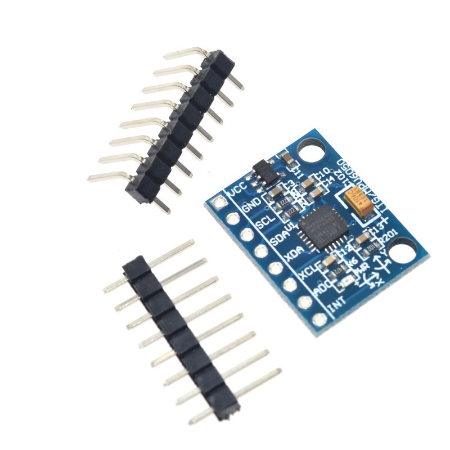
\includegraphics[width=8cm]{MPU}
\caption{Modul GY-521\cite{GY-521pic}}
\label{fig:MPU}
\end{figure}
Riešenie problému merania uhla u pohybujúceho sa robota predstavuje kombinácia nameraných hodnôt z akcelerometra a gyroskopu, pomocou komplementárneho filtra. Na toto využite sa hodí modul GY-521 obsahujúci senzor MPU 6050\cite{MPU6050datasheet}, ktorý v sebe kombinuje trojosový akcelerometer a gyroskop. Modul je schopný komunikovať s mikropočítačom pomocou rozhrania I2C maximálnou rýchlosťou 400kHz a obsahuje taktiež integrovaný teplomer a DMP (Digital Motion Processor).Ten je schopný priamo uskutočniť analýzu nameraných dát, čím sa znížia požiadavky na výpočtový čas mikropočítača.



\subsection{Riadiaci počítač - Arduino MEGA}
Vďaka skúsenostiam s programovaním mikropočítačov spoločnosti Microchip-Atmel sme sa pri výbere mikropočítača rozhodovali medzi mikropočítačmi rodiny ATMEGA. Do úvahy prichádzali hlavne ATMEGA328P\cite{ATMEGA328} a ATMEGA2560\cite{ATMEGA2560}, ktorých výpočtové možnosti a zabudované periférie postačovali našim požiadavkám. Jednou zo zvažovaných možností bolo navrhnutie a skonštruovanie obvodu so zabudovaným mikropočítačom, ktorý by priamo zodpovedal požiadavkám našej aplikácie. Toto riešenie sme ale nakoniec po úvahe zavrhli, keďže by bolo časovo náročné a nespadalo by do koncepcie modularity – takto navrhnutý obvod by v prípade poruchy bol náročný na nahradenie a bolo by veľmi náročné upraviť ho pri zmene požiadaviek na robota.

Rozhodli sme sa teda využiť rozšírenú otvorenú vývojovú platformu Arduino, ktorá vo všeobecnosti slúži na vývoj prototypov a testovanie kódu. Našou voľbou bolo Arduino MEGA \figurename~\ref{fig:arduinoMega}, využívajúce mikropočítač ATMEGA2560. Táto vývojová doska má zabudovaný programovací port USB typu B (ktorý sme zamenili na micro USB), napäťový regulátor na 5V a 3.3V, 16 MHz oscilátor (zdroj hodinového signálu pre mikropočítač) a na rozdiel od lacnejšieho Arduino Uno má až 53 GPIO (General Purpose Input Output) pinov, 16 pinov podporujúcich ADC (prevod analógového signálu na jeho digitálnu reprezentáciu) a 6 pinov podporujúcich niekoľko režimov prerušení.

\begin{figure}[h]
\centering
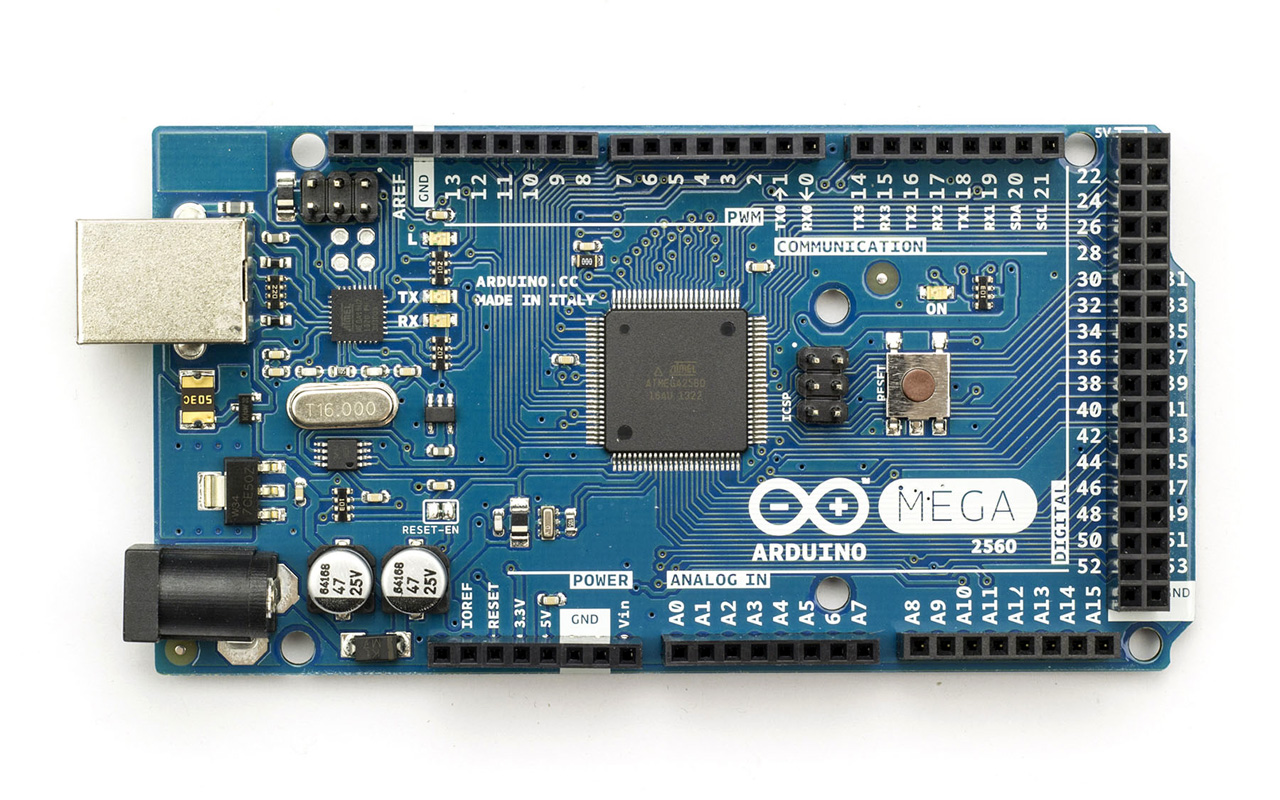
\includegraphics[width=8cm]{arduinoMega}
\caption{Arduino Mega\cite{arduinoMEGA}}
\label{fig:arduinoMega}
\end{figure}

Samotný mikropočítač má viacero časovačov, ktoré umožňujú napr. merať časové intervaly a generovať PWM signál, ale taktiež 4 páry RX, TX pinov slúžiacich na komunikáciu pomocou UART protokolu. Ako ďalšie možnosti komunikácie je možné využiť aj I2C a SPI protokoly. Programovanie dosky Arduino MEGA je možné cez USB rozhranie, napr. pomocou programu ArduinoIDE, AtmelStudio alebo Eclipse. Našou voľbou bolo využitie všestranného editora Eclipse, v kombinácii s pluginom umožňujúcim jednoduchú prácu s mnohými produktami Microchip-Atmel.



\section{Návrh a výroba šasi robota}
Pri výrobe šasi robota sme sa rozhodli použiť technológiu 3D tlače. S jej použitím sme boli schopný vytvoriť pevné a ľahké šasi, ktoré presne zodpovedalo našim požiadavkám. Pred samotnou tlačou sme ale museli navrhnúť model v CAD programe tak, aby bolo nielen jednoduché ho vytlačiť, ale aj aby bolo schopné odolať nárazom a ochrániť tak elektroniku vo vnútri. Pri návrhu sme použili software Fusion 360, ktorý je pre študentov dostupný zdarma na stránke firmy \href{https://www.autodesk.com/products/fusion-360/overview}{Autodesk}.

Program Fusion 360 podporuje ako návrh a export modelov do viacerých bežne používaných formátov, tak aj analýzu vlastností modelu, simuláciu jeho správania pri záťaži, nástroje na vizualizáciu, animáciu a mnoho ďalších užitočných funkcií.

Nami vytvorené šasi  sa skladá z dvoch častí a to veka a miskovitého tela, v ktorom sú uložené komponenty. Po naštudovaní prác, ktoré už boli na tému návrhu dvojkolesového balansujúceho robota napísané, sme zvolili pre celé šasi klinovitý tvar s úzkou podstavou a širokých vrchom. Tento tvar nám umožní jednoduché napojenie servomotora na spodnú časť robota a osadenie batérie blízko k hornej časti robota. V takomto usporiadaní dosiahneme relatívne vysoko umiestnené ťažisko, čo následne zjednoduší stabilizovanie robota. Šasi taktiež obsahuje otvory na kabeláž od motorov, dve LED diódy indikujúce stav robota, spínač napájania a prístup k portu micro USB, vďaka ktorému je možné robota programovať bez nutnosti demontáže veka.

Tlač prebehla po vytvorení gcode súboru v nástroji Cura na tlačiarni Creality CR-10s. Na tlač bol použitý materiál PLA (Polyactic Acid), ktorý sa vyznačuje nízkou tepelnou rozťažnosťou pri chladnutí, nízkou cenou a jednoduchou tlačou. 

\begin{figure}
\centering
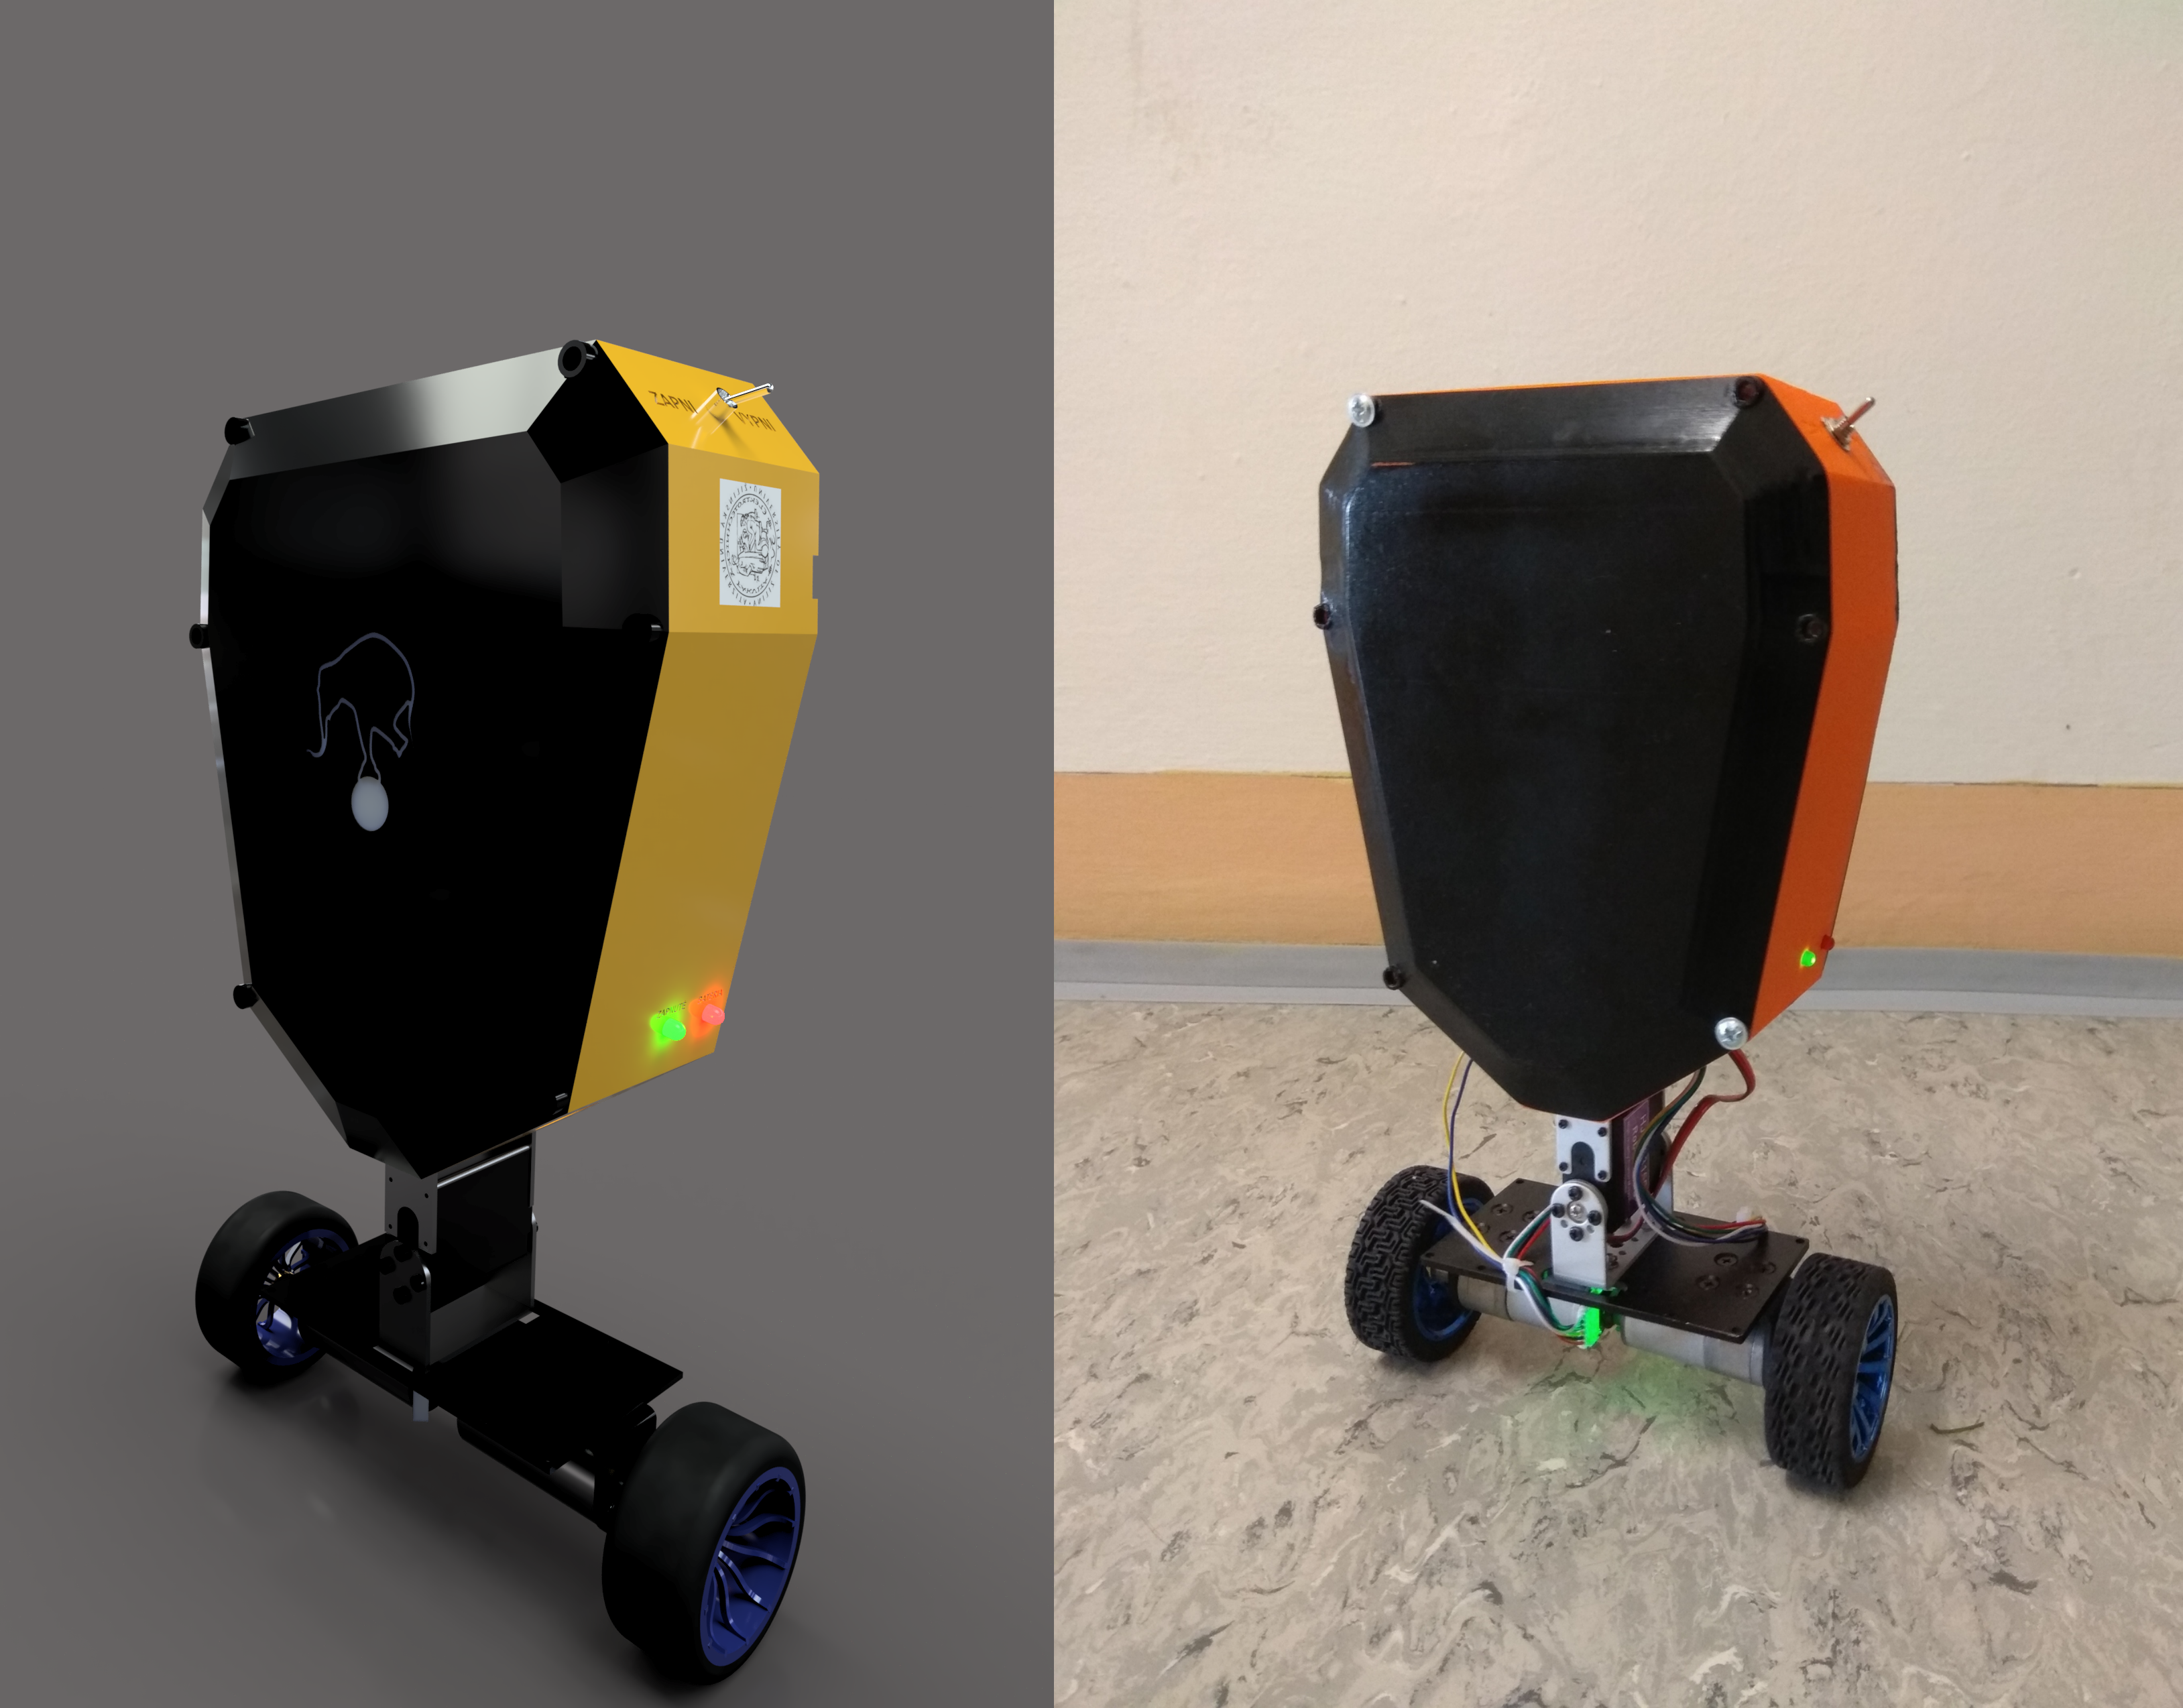
\includegraphics[width=14cm]{robotComp}
\caption{Porovnanie modelu a reálnej podoby robota}
\label{fig:robotComp}
\end{figure}

Samotná tlač trvala približne až 50 hodín, kvôli požiadavke na relatívne vysokú presnosť (a teda malú výšku jednotlivých vrstiev), pričom sa pri nej spotrebovalo približne $0,5~kg$ PLA. Po vytlačení, osadení komponentov a nalakovaní sa nami vytvorený model výzorom blížil k jeho počítačovo vygenerovanej podobe viď. \figurename~\ref{fig:robotComp}. Po kontrole môžeme tiež konštatovať, že vnútorné a vonkajšie rozmery oboch dielov presne zodpovedali nášmu návrhu.

Pri tlači sa vyskytli menšie chyby, ktoré spôsobili artefakty na veku robota v podobe pruhov spôsobených krycou páskou na podstave tlačiarne. Ako problematické sa ukázalo taktiež vytlačenie tela, na ktorého povrchu boli po vytlačení viditeľné chyby v podobe nezaplnených miest a príliš zaoblených hrán. Tie mohli byť spôsobené nesprávnym nastavením parametrov v programe Cura, privysokou teplotou vyhrievanej podstavy tlačiarne alebo príliš priľnavou podstavou. 

Výsledné výtlačky boli ale použiteľné, keďže vyššie opísané chyby boli čisto estetického charakteru. Ako závažnejším problémom sa ukázala realizácia kabeláže. Napriek dostatku miesta bolo po zapojení všetkých komponentov náročné sa v kabeláži vyznať, čo by mohlo spôsobiť problémy pri dodatočnej údržbe. 

Na vyriešenie tohto problému sme navrhli a dali vyhotoviť tzv. shield. Tento shield je doska plošných spojov, ktorá svojim vyhotovením predstavuje nadstavbu Arduina. Takýto shield je možné jednoducho pripojiť k Arduinu a jeho výhodou je tiež, že môže obsahovať označené terminály, umožňujúce bezpečné pripojenie komponentov k Arduinu. 

\begin{figure}[h]
\centering
\begin{minipage}[b]{0.48\textwidth}
\centering
\includegraphics[width=\textwidth]{robotInsideFoto}
\caption{Pred osadením shieldu}
\label{fig:robot_no_shield}
\end{minipage}\quad
\begin{minipage}[b]{0.48\textwidth}
\centering
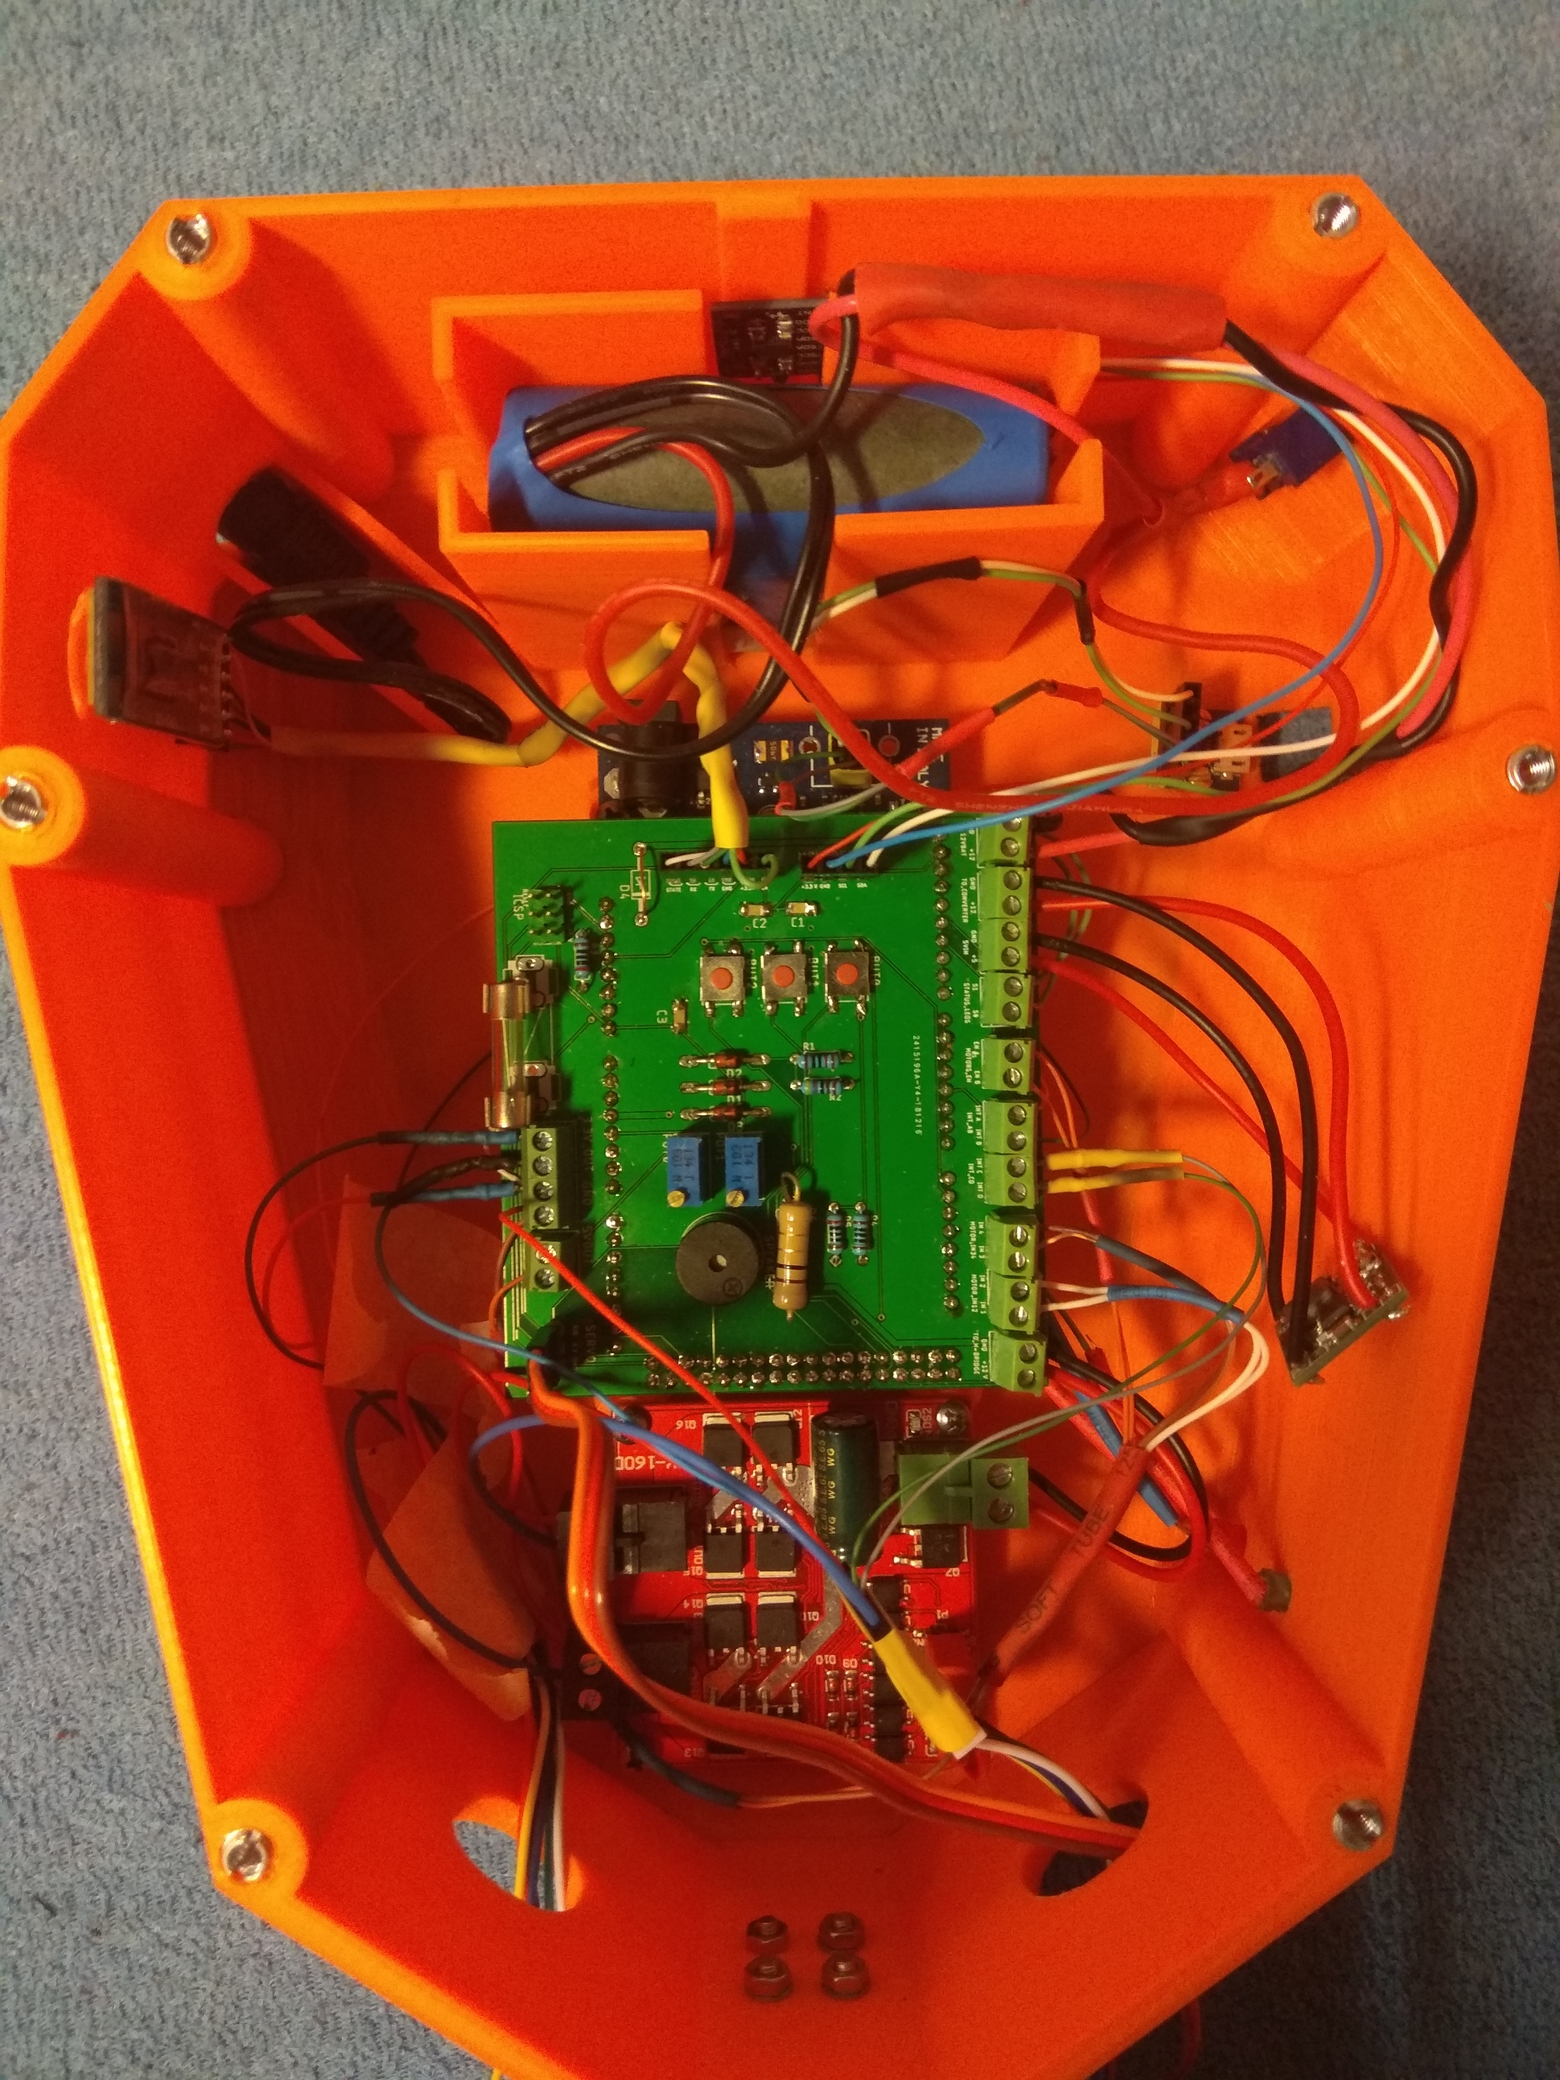
\includegraphics[width=\textwidth]{shield}
\caption{Po osadení shieldu}
\label{fig:robot_shield}
\end{minipage}
\label{fig:comparison}
\end{figure}

Návrh tejto dosky plošných spojov sme uskutočnili v bezplatnej verzii nástroja Eagle. Tá umožňuje návrh elektrických schém aj PCB (Printed Circuit Board) a generovanie gerber súborov, ktoré obsahujú informácie pre výrobcu. Ukážka takto vytvorenej dosky je v prílohe \figurename~\ref{fig:neosadenyShield}, pričom pri jej tvorbe sme vychádzali zo schémy na \figurename~\ref{fig:schemaShield}. 

Zo schémy je zjavné, že nami vytvorený obvod obsahuje okrem vstupno/výstupných terminálov aj dodatočnú ochranu vstupov proti prepätiu. Táto je realizovaná formou Zenerových diód s hodnotou prierazného napätia 5 V, zapojených v závernom smere. Napriek tomu, že mikropočítač ATmega 2560 obsahuje zabudované diódy, ktoré vedia vstupy ochrániť proti krátkodobému prepätiu, externé zenerove diódy prejdú do vodivého stavu skôr a zabránia tak prípadnému poškodeniu mikropočítača prepätím. 

Medzi ďalšie ochranné prvky, ktoré sme implementovali, patrí Shottkyho dióda zapojená do série s batériou, ktorá zabráni poškodeniu komponentov v prípade nesprávneho pripojenia batérie. Podobným spôsobom zapojená tavná poistka ochráni batériu pred možným skratom v obvode.  Keďže bluetooth modul, ktorý sme zvolili pre realizáciu komunikácie, pracuje s logickými úrovňami od $0 V$ do $3,3 V$, ale Arduino výstupy pracujú s $5 V$, pripojili sme RX vstup modulu k mikropočítaču cez napäťový delič. 

Doska plošných spojov obsahuje aj dva potenciometre, tri spínače a reproduktor. Potenciometre a spínače budú v prípade potreby slúžiť na jemnú kalibráciu alebo manuálne zadávanie jednoduchých povelov. Reproduktor so zabudovaným oscilačným obvodom slúži ako hlásič, napr. v prípade prebiehajúcej kalibrácie. Kompletná schéma nami navrhnutého shieldu je v prílohe na \figurename~\ref{fig:schemaShield}. Porovnanie vnútra robota pred a po osadení shieldu je na \figurename~\ref{fig:robot_no_shield}, \figurename~\ref{fig:robot_shield}.

\section{Výsledky montáže a zhodnotenie návrhu}
Nami navrhnutý dizajn robota sa v praxi ukázal ako veľmi jednoduchý na skonštruovanie. Po vytlačení šasi robota na 3D tlačiarni stačilo len spojiť skrutkami servo, šasi a podvozok robota a následne zrealizovať kabeláž podľa schémy \figurename~\ref{fig:schemaShield}.Finálny vzhľad robota po zmontovaní je na \figurename~\ref{fig:robot_front} \figurename~\ref{fig:robot_side}. Do vnútra šasi robota sme bez problémov nainštalovali všetky potrebné komponenty a ponechali dostatok voľného miesta na prípadné neskoršie úpravy robota.   

\begin{figure}[h]
\centering
\begin{minipage}[b]{0.48\textwidth}
\centering
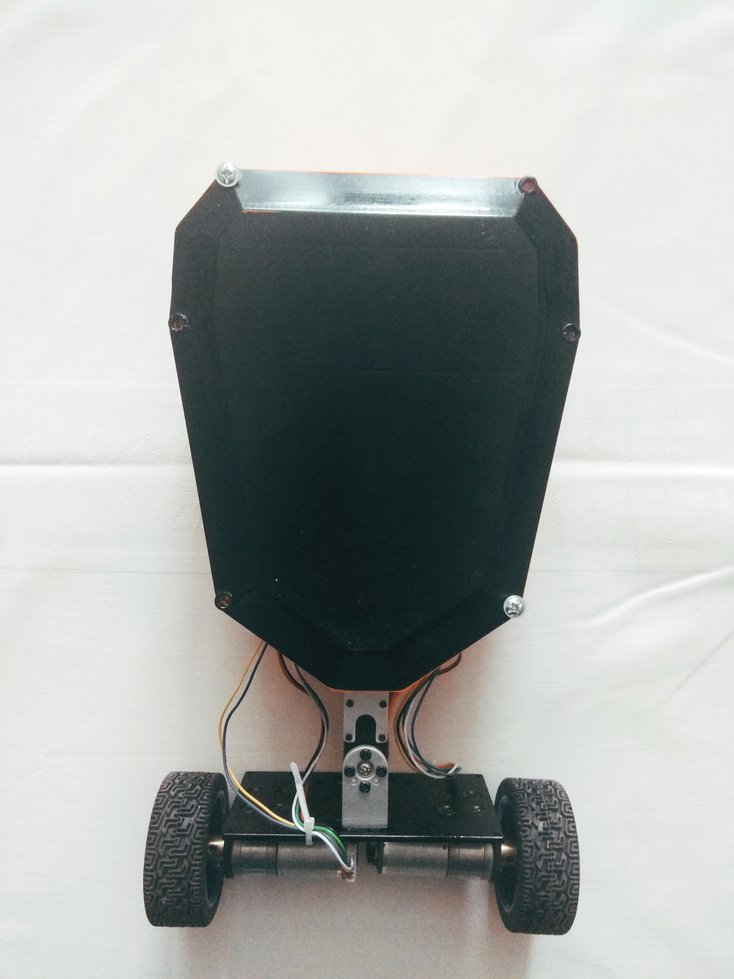
\includegraphics[width=\textwidth]{front_robot}
\caption{Robot spredu}
\label{fig:robot_front}
\end{minipage}\quad
\begin{minipage}[b]{0.48\textwidth}
\centering
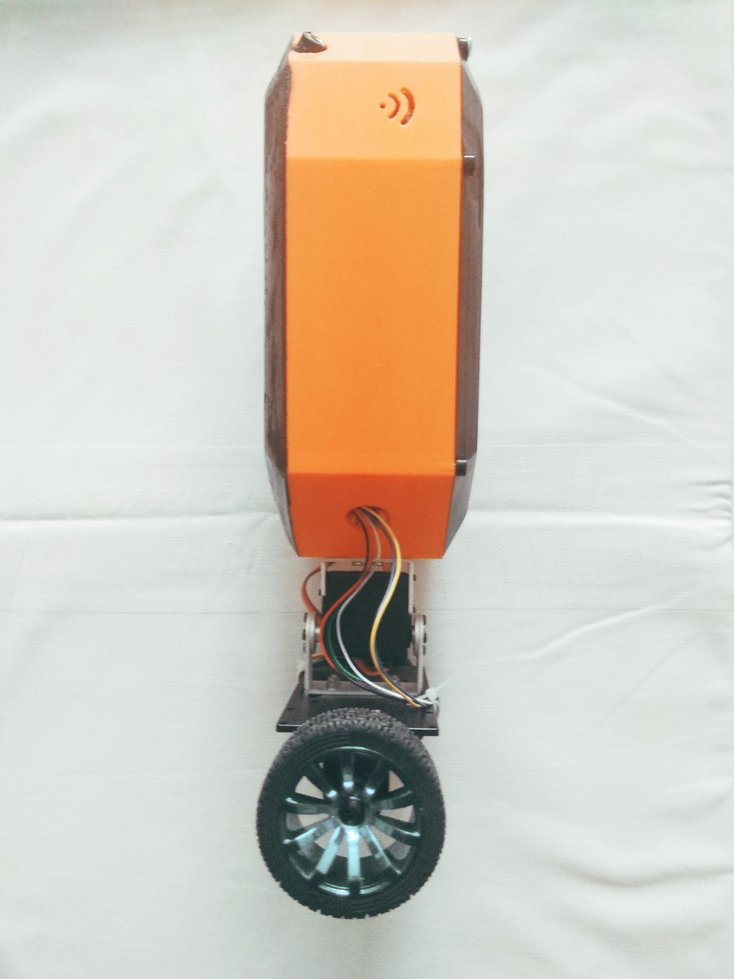
\includegraphics[width=\textwidth]{side_robot}
\caption{Robot zboku}
\label{fig:robot_side}
\end{minipage}
\end{figure}

Pri motáži sme ale identifikovali niekoľko nedostatkov nášho návrhu. Jedným z nich bolo nevhodné umiestnenie senzora MPU6050 priamo nad batériou, čím sme značne limitovali možnosti prístupu k senzoru po montáži. Samotný priestor pre osadenie batérie bol pôvodne navrhnutý bez veka, ktoré by zabránilo batérií v pohybe pri činnosti robota. Navrhnúť vhodné veko sa ale ukázalo ako značne náročné. Dôsledkom toho bolo, že batéria musela byť ukotvená použitím lepidla, čo nie je najvhodnejšie riešenie, pretože značne komplikuje prípadnú výmenu batérie za iný model.    

\section{Návrh a výroba ovládača robota}

Pri návrhu ovládača robota sme postupovali podobným spôsobom ako pri návrhu šasi. Rovnako ako pri šasi aj tu bol na návrh ovládača použitý nástroj Fusion 360 a technológia 3D tlače. Takto navrhnutý ovládač obsahuje dvojosový analógový joystick, ktorý riadi pohyb robota a umožňuje používateľovi pohyb v menu nastavení. Informácie získava používateľ zo zabudovaného 1,8 palcového farebného TFT displeja. Orientáciu v menu zjednodušujú dve zabudované tlačidlá.

\begin{figure}[h]
\centering
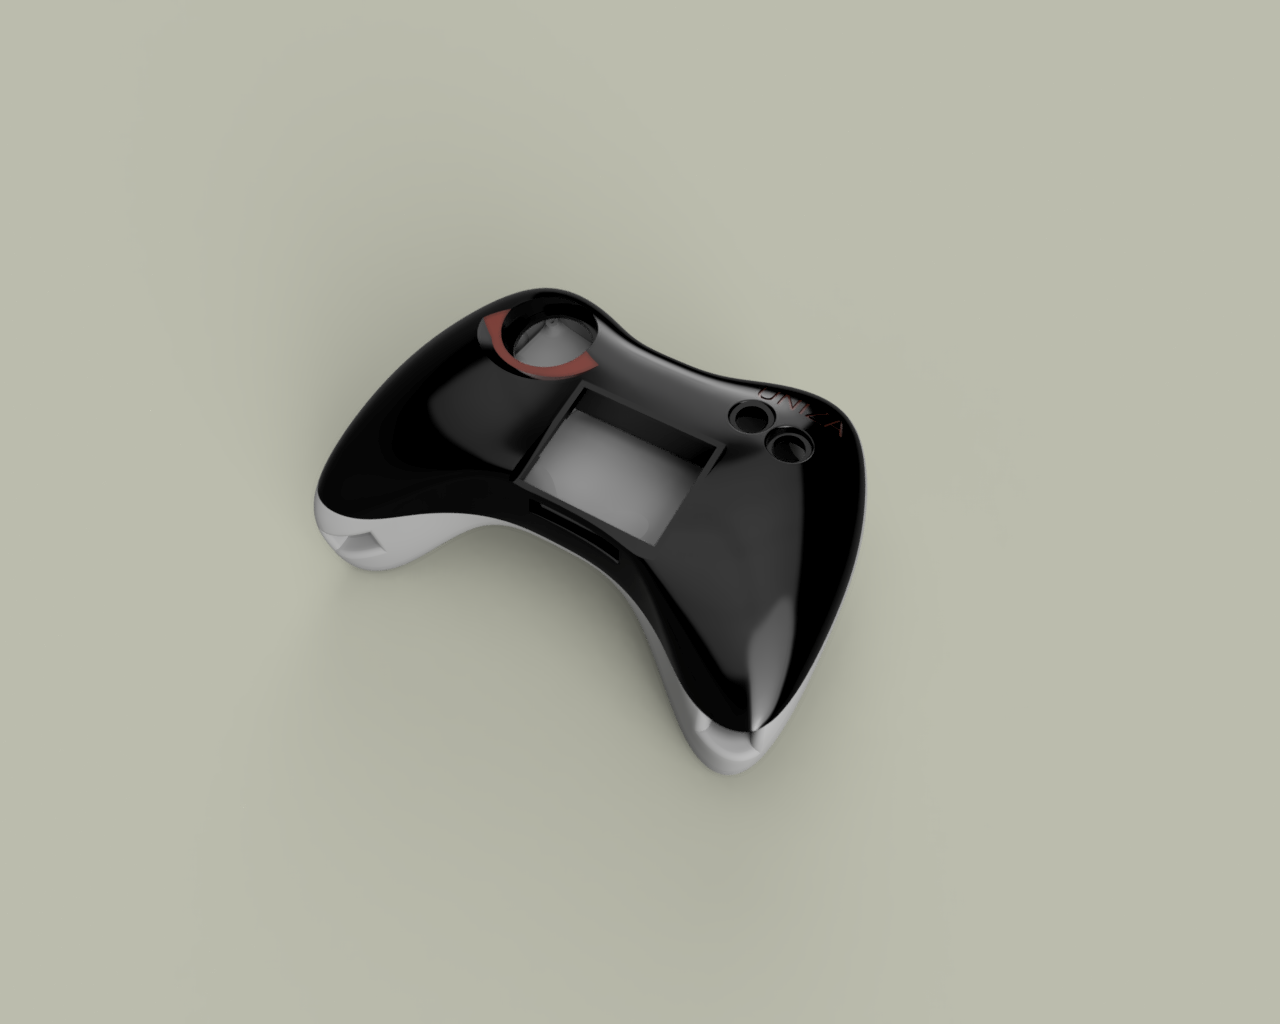
\includegraphics[width=8cm]{kontrolerVizu}
\caption{Ovládač balansujúceho robota}
\label{fig:kontrolerVizu}
\end{figure}

Napájanie ovládača je riešené z klasickej 9V batérie, zredukovanej spínaným zdrojom na $5V$ a na samotnú komunikáciu slúži modul HC-05 spomenutý v prvej časti tejto kapitoly. Okrem vysielania riadiacich príkazov ovládač v periodických intervaloch prijíma od robota dáta o jeho stave, ktoré následne zobrazuje užívateľovi na displeji.
 
Ovládač je schopný zobraziť informácie o uhle náklonu robota, aktuálnej rýchlosti, priemernej rýchlosti, aktuálnych kalibračných hodnotách a stave batérie. Používateľ môže taktiež prostredníctvom ovládača dať robotovi pokyn na začatie autokalibrácie a odoslanie dát do počítača cez sériový port.

Na rozdiel od predchádzajúceho prípadu, kedy sme navrhli okrem šasi taktiež dosku plošných spojov, v prípade ovládača neexistujú požiadavky na nijakú dodatočnú elektroniku a tak táto potreba odpadá. Komponenty budú spojené vnútri ovládača priamo s vývojovou doskou Arduino Nano. Malé rozmery tejto dosky zabezpečia, že rozmery ovládača budú podobné bežne predávaným konzolovým ovládačom. 

Ako problematická sa ukázala spotreba spínaného regulátora napätia, ktorá  bola v prípade nezaťaženého regulátora až $8 mA$. Takýto trvalý odber by nami použitú batériu rýchlo zničil, pristúpili sme teda k priradeniu spínača, ktorým bude batériu možné priamo odpojiť, keď bude ovládač nepoužívaný.


\chapter{Návrh a implementácia riadiaceho systému robota.}
Základom nami použitého riadiaceho systému boli dva PID regulátory zapojené do kaskády. Toto zapojenie budeme ďalej označovať ako \ac{RS}. Vstupom RS je požiadavka na rýchlosť pohybu robota v $rad.s^{-1}$ a výstupom strieda PWM signálu privádzaná na vstup do H-mostíka, vyjadrená hodnotou od -100\% až 100\% (kde záporná hodnota predstavuje zmenu smeru otáčania motorov). Funkcia jednotlivých PID regulátorov v RS bude vysvetlená v nasledujúcej časti práce. Je nutné podotknúť, že samotné zabezpečenie balansovania robota na mieste je možné realizovať použitím jediného PID regulátora. Nevýhodou takéhoto postupu je ale nemožnosť akejkoľvek regulácie rýchlosti pohybu robota. 

\section{Štruktúra RS robota}

Na \figurename~\ref{fig:RS} sme znázornili zapojenie PID regulátorov v RS.  

\begin{figure}[h]
\centering
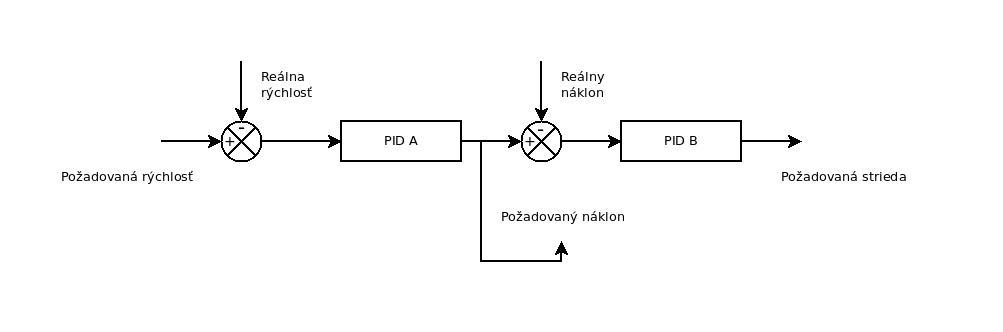
\includegraphics[width=10cm]{PID_robota}
\caption{Schematické zapojenie PID regulátorov}
\label{fig:RS}
\end{figure}

\underline{\textbf{PID A}}:
Vstupom do PID A je požadovaná rýchlosť robota, tá je následne odčítaná od reálnej rýchlosti nameranej pomocou enkodérov a spracovaná PID regulátorom. Pri riadení robota môžeme špecifikovať požadovanú rýchlosť a na výstupe PID A bude požadovaný uhol náklonu. Týmto spôsobom zabezpečíme ako dosiahnutie požadovanej rýchlosti, tak aj to, že robot sa bude pohybovať konštantnou rýchlosťou. Výhodnou vlastnosťou PID A je, že požadovaný uhol náklonu nebude počas celej doby riadenia konštantný pre danú rýchlosť, ale bude dynamicky prispôsobovaný aktuálnym podmienkam. Ak by to tak nebolo robot by pri konštantnom uhle náklonu pokračoval v zrýchľovaní aby sa vyhol pádu až pokiaľ by motory dosiahli maximálnu rýchlosť a neboli schopné dosiahnuť požadované zrýchlenie na udržanie uhla náklonu. Po tomto bode by nasledoval pád.

\underline{\textbf{PID B}}:
Výstupom PID B je ako už bolo skôr spomenuté strieda signálu vstupujúceho do H-mostíka. V prípade nami použitého mostíka platí priama úmera medzi striedou vstupného signálu a napätím do motorov. Nedá sa ale povedať, že by závislosť medzi striedou a výstupným napätím bola lineárna. V skutočnosti pre efektívne napätie na výstupe mostíka platí vzťah \eqref{eq:RMSSquare}, v ktorom $\delta$ je z intervalu $<0;1>$ a predstavuje striedu vstupného signálu. Závislosť výstupného napätia a striedy je zobrazená na \figurename~\ref{fig:strieda_napatie}. V našom prípade sa ale nejedná o závažný nedostatok, ktorý by výrazným spôsobom ovplyvňoval výsledky regulácie.

\begin{equation}
U_{EF} = U_{MAX}\sqrt{\delta}
\label{eq:RMSSquare}
\end{equation}

\begin{figure}[b]
\centering
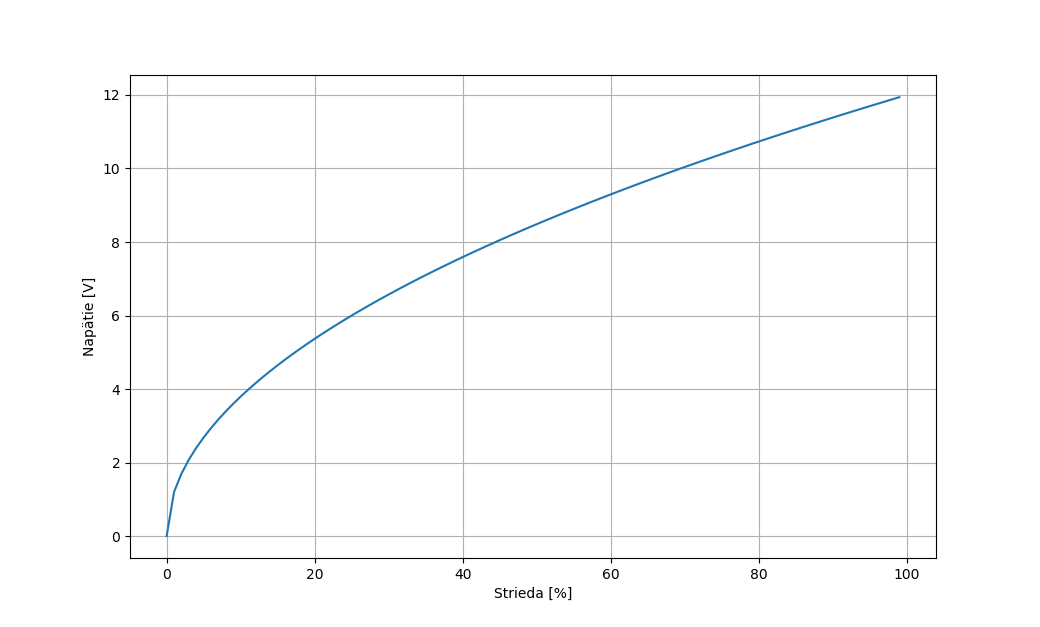
\includegraphics[width=10cm]{strieda_napatie}
\caption{Znázornenie závislosti medzi striedou a napätím}
\label{fig:strieda_napatie}
\end{figure}

Ladenie \ac{RS} prebiehalo po častiach. Ako prvý sme naladili PID B, pričom využitá bola Zieger-Nicholsova metóda, nasledovaná jemným, manuálnym doladením parametrov. Pri ladení bol na vstup privedený nulový vstupný signál, reprezentujúci požiadavku na nulový uhol náklonu. Výsledkom tohto ladenia bol robot schopný balansovať vo vzpriamenej polohe a taktiež odolať aj silnejším pokusom o jeho prevrhnutie. Ako nedostatkom sa ale javilo to, že robot nebol nijakým spôsobom penalizovaný za pohyb a tak trvalo aj niekoľko sekúnd kým sa po postrčení opäť dostal do ustáleného stavu (stav charakterizovaný minimálnou osciláciou okolo osi natočenia a minimálnou rýchlosťou pohybu).

Po naladení PID B, bol ladený PID A, pričom sme na vstup RS opäť priviedli nulovú hodnotu - teda požiadavku na nulovú rýchlosť. Keďže pri prevádzke bude práve tento stav s nulovou požiadavkou najčastejší pri ladení PID A sa kládol silný dôraz na správanie systému pri návrate do ustáleného stavu. PID A bol naladený obdobným spôsobom ako PID B. Výsledkom bol \ac{RS} schopný zabezpečiť minimálnu uhlovú výchylku robota pri minimálnej rýchlosti pohybu.

Keďže pri realizáciu PID bola použitá forma popísaná v \ref{eq:compPID} bolo ešte potrebné určiť konštantu $T_f$ podľa vzťahu \ref{eq:TFconst}. Pri zisťovaní oscilačnej frekvencie robota pri pohybe sme na presné zmeranie krátkych periód oscilácií použili kamerový záznam pohybu robota. Pri známej frekvencií snímkovania, ktorá bola v našom prípade 60 \ac{FPS} (frames per second), je spočítaním snímok a ich vynásobením periódou snímkovania možné presne odmerať aj krátke časové okamihy. Zavedenie konštanty $T_f$ zlepšilo vlastnosti \ac{RS} robota.

Takto naladené PID regulátory pracujú v zapojení do kaskády, pričom PID B pracuje s periódou 10ms a PID A s periódou 50ms. Tento čas je dostatočný na to aby bol robot schopný rýchlo reagovať na podnety a dostatočne dlhý na to aby sme mohli získať a spracovať dáta zo senzorov. Dôvodom relatívne dlhej periódy PIDu B je princíp fungovania enkodéra, z ktorého by sme pri výrazne kratšej perióde meraní neboli schopný získať presné dáta.   

\section{Implementácia riadiaceho systému}
Implementácia \ac{RS} robota bola realizovaná v jazyku C++, pričom sme využili objektovo orientovaný spôsob programovania. V praxi to znamená, že jednotlivé funkčné celky robota sú reprezentované v dátových štruktúrach nazývaných objekty. Každý objekt predstavuje inštanciu triedy, v ktorej sú definované jeho vlastnosti a metódy - teda jeho štruktúra. Prostredníctvom týchto vlastností a metód objekt vykonáva v rámci funkčného celku určité funkcie. Výhodou tohto postupu je, že takto napísaný kód je znovu použiteľný aj v iných projektoch a v prípade potreby jednoducho rozšíriteľný o dodatočnú funkcionalitu. Zapuzdrenie jednotlivých funkčných celkov taktiež pomáha udržiavať kód prehľadný.

Príkladom triedy v nami použitom kóde je napríklad trieda \textit{PID}. V tejto triede sú definované metódy, ktoré by mal byť každý objekt triedy PID schopný realizovať. V našom prípade sa jedná o metódy pre nastavenie a úpravu parametrov P, I, D a metódu pre vypočítanie výstupe PIDu vzhľadom na určitý vstup. Vytvorenie tejto triedy nám umožnilo reprezentovať PID A a PID B ako inštancie tejto triedy. 

Pri triede PID je treba poznamenať, že priame použitie \ref{eq:compPID} na vypočítanie výstupu by nebolo možné, keďže v nami predstavenej forme sa jedná o spojitý regulátor. Mikroprocesor je ale digitálne zariadenie, ktoré nie je schopné priamo realizovať spojitú funkciu, ani prijímať spojité dáta (ktoré by väčšina nami použitých senzorov ani nebola schopná poskytnúť). Je preto potrebné vyjadriť \ref{eq:compPID} aj vo spojitej forme. Výstup PID pre vzorku číslo $i$ je teda:
\begin{equation}
y_i = Pe_i + I\sum_{k=0}^{i}{e_k}\Delta t + D\Delta e_i 
\end{equation}
pričom $e_i$ je rozdiel požadovaného uhla a skutočného uhla, pre vzorku $i$, $\Delta t$ je čas medzi jednotlivými vzorkami a $\Delta e_i$ je možné vyjadriť ako:
\begin{equation}
\Delta e_i = \dfrac{T_f\Delta e_{i-1} + (e_i - E_{i-1})}{\Delta t + T_f}
\end{equation}


\listingname~\ref{lst:PIDsample} predstavuje ukážku jednej nami implementovanej metódy triedy PID. Jej výstup predstavuje výstup daného PID regulátora.  


\begin{inlinecode}[label={lst:PIDsample},caption={Príklad jednej z metód triedy PID}]{c++}
float PID::giveOutput(float input, float target, float dt, float constrainI){
    float output  = 0;
    float Perror = target-input;
    error_integral += Perror;
    if(constrainI){
        error_integral = constrain(error_integral,-constrainI,constrainI);
    };
    error_derivative = (Tf*error_derivative + (Perror - old_error))/(dt + Tf);       //implements filtering constant Tf
    output = P*(Perror)+I*(error_integral)*dt+D*error_derivative;

    old_error = Perror;
    return output;
}
\end{inlinecode}

Celý nami vytvorený kód pracuje po úvodnej inicializácií premenných a vytvorení objektov na princípe kontrolnej slučky, t.j. skupiny príkazov, ktoré sa periodicky opakujú. V našom prípade sme túto slučku navrhli tak aby prebehla raz za každých 10 ms. V tejto riadiacej slučke načítavame nové údaje zo senzorov, spracovávame ich prostredníctvom \ac{RS} a na vstup H-mostíka privádzame výsledný signál \ac{PWM}. Celý proces je znázornený v diagrame \figurename~\ref{fig:simpleFlowchart}.

V \figurename~\ref{fig:simpleFlowchart} nie sú znázornené spracovania prerušení, v ktorých sa spracúvajú údaje z enkodérov, použitých na monitorovanie aktuálnej rýchlosti robota. Výstup zo samotných enkodérov prichádza do mikropočítača po štyroch dátových linkách (dve pre každý enkodér), vo forme impulzov vzájomne oneskorených o čas $t_e$. Výstup z dvoch kanálov enkodéra je zobrazený na \figurename~\ref{fig:enkoder}. Na jedinú otáčku kolesa pripadá $N$ takto vzájomne posunutých impulzov (pre jeden kanál). Spočítaním týchto impulzov za čas  $t_S$ vieme určiť uhlovú rýchlosť kolesa $\omega$ a z nej následne odvodiť celkovú rýchlosť pohybu robota. Smer pohybu určíme podľa poradia detekcie impulzov. Vzorec pre výpočet rýchlosti pohybu robota je teda možné vyjadriť ako:
\begin{align*}
\Delta\phi_w &= \dfrac{2\pi}{N}k \qquad [rad] \\
\omega &= \dfrac{\Delta\phi_w}{t_S} \qquad [rad.s^{-1}]\\
v &= \omega r \qquad[m.s^{-1}]
\end{align*}
kde $\Delta\phi_w$ predstavuje zmenu uhla natočenia kolesa $k$ predstavuje počet detegovaných impulzov z jednej linky za čas $t_S$ a $r$ polomer kolesa robota.

Následne je ešte potrebné zredukovať šum prítomný v takto nameraných dátach, v našom prípade pomocou komplementárneho filtra. Komplementárny filter bol taktiež použitý aj pri filtrovaní a fúzií dát nameraných z akcelerometra a gyroskopu.  

Podrobná schéma zobrazujúca celkovú činnosť \ac{RS} robota je na \figurename~\ref{fig:podrobna_schema}. Znázorňuje ako RS robota, tak aj spôsob spracovania dát na jeho vstupoch.
\begin{figure}[!b]
\centering
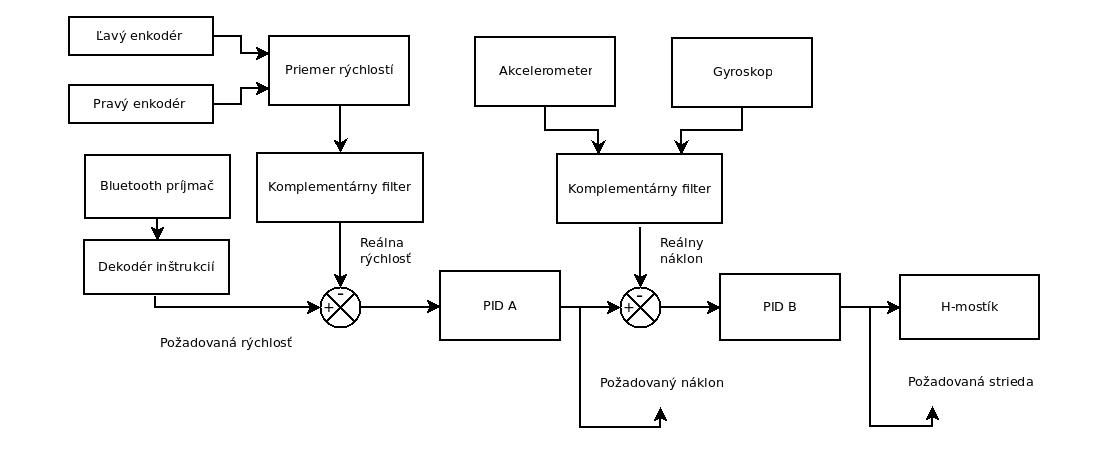
\includegraphics[width=15cm]{comp_RS_diagram}
\caption{Podrobná schéma RS robota}
\label{fig:podrobna_schema}
\end{figure}

Zaujímavosťou je, že pri fúzií dát z gyroskopu a akcelerometra sa ukázalo ako výhodné v komplementárnom filtri s postupom času potláčať vplyv merania z akcelerometra až po dosiahnutie určitej konečnej hodnoty. Dôvodom je, že pri spustení potrebuje robot chvíľu na to aby presne zistil svoj uhol natočenia, tento môže presne získať len z akcelerometra. Po zorientovaní a správnom nastavení polohy je výhodné potlačiť vplyv akcelerometra čím sa zamedzí vplyvu náhodných otrasov a silných postrčení na presnosť merania uhla (akcelerometer je na tieto omnoho citlivejší ako gyroskop).

\section{Ovládanie pohybu robota}
Použitím komunikačného rozhrania využívajúceho technológiu Bluetooth sme zabezpečili jednoduchú a dostatočne rýchlu komunikáciu medzi robotom a ovládačom, prostredníctvom ktorého je operátor schopný jednoducho zadávať robotovi príkazy. Následne ale bolo potrebné zabezpečiť aby sa tieto príkazy spoľahlivo premietali do riadenia pohybov robota. Taktiež bolo potrebné zabezpečiť aby robot nebol závislí od príkazov operátora a dokázal balansovať na mieste aj bez prítomnosti riadiaceho signálu.

Riadiaci signál prichádzajúci z ovládača prenáša riadiace príkazy vo forme jednotlivých bajtov, pričom prvý bajt slúži ako jedinečný identifikátor príkazu. Takýmto spôsobom sme zabezpečili jednoduché odlíšenie až 256 jedinečných príkazov, ktoré robot môže od ovládača prijať. V prípade príkazu prenášajúceho pohybové povely bude tento prvý jedinečný identifikátor nasledovaný dvoma bajtami dát, ktoré obsahujú preškálované hodnoty z 10-bitového prevodníka ADC v ovládači, napojeného na X-ovú a Y-ovú os analógového joypadu.  

Dosiahnutie plynulého riadenia rýchlosti po prijatí riadiaceho bajtu, bolo jednoduché. Hodnota prijatá z X-ovej osi joypadu sa preškáluje z rozsahu 0-100 na $-v_d$ až $v_d$. Túto hodnotu po preškálovaní ozn. $v_s$ a použitá je ako vstup do PID A. Po praktickom testovaní rôznych hodnôt $v_d$ sme vo finálnej verzií robota použili hodnotu $v_d = 7$. V praxi hodnota $v_d$ predstavuje max. rýchlosť pohybu robota v $rad.s^{-1}$.

Praktické testy ďalej ukázali, že pred vložením vypočítanej rýchlosti $v_s$ na vstup PID A je vhodné použiť komplementárny filter, ktorý spomalí rýchlosť nárastu $v_s$. Týmto postupom sme docielili plynulejšie zrýchlenie a spomalenie robota, čo v konečnom dôsledku prispelo k celkovému zlepšeniu stability robota.

Ako problematické sa v praxi ale ukázalo riadenie smeru robota. Pri prvých pokusoch sme prijatú hodnotu z Y-osi joypadu preškálovali a filtrovali spôsobom analogickým ako pri riadení rýchlosti a takto získanú hodnotu $o_s$ sme používali pri riadení motorov. V prípade ľavotočivej zatáčky tak bola k hodnote požadovanej striedy pravého motora pripočítaná hodnota $o_s$ a od striedy ľavého odpočítaná (opačne pre pravotočivú zatáčku). Tento systém spoľahlivo pracoval pri rozbehnutom robotovi, ale ukázal sa ako nedostatočný pri pokusoch otáčať nehybného robota.

Problémom pri otáčaní nehybného robota bol fakt, že v skutočnosti nie je možné dosiahnuť balansovanie robota bez rýchlych zmien striedy vstupujúcej do H-mostíka. Tieto zmeny striedy sú natoľko rýchle, že v praxi sa prejavia len jemným chvením robota, ale pri snahe upravovať striedu o hodnotu $o_s$ dôjde len k trhaným pohybom robota na mieste. Tento nedostatok sa nám nepodarilo odstrániť ani zmenou parametrov komplementárneho filtra ani zmenami $o_s$.

Ako uspokojivé riešenie sa nakoniec ukázalo riadenie zatáčania za jazdy pomocou $o_s$ a riadenie otáčania na mieste priamym zavedením predefinovanej striedy na oba motory, podľa požadovaného smeru otáčania a pri dodržaní maximálnej dovolenej rýchlosti robota, pri ktorej je ešte možné otočku vykonať. Pri tomto spôsobe otáčania ostáva strieda motorov po určitý, krátky čas stabilná a dostatočne veľká na to, aby spôsobila otočenie robota na mieste bez výrazného narušenia jeho stability. 

\section{Podporné metódy riadenia}
Pri testovaní RS sme zvažovali aj niektoré ďalšie, podporné, metódy riadenie správania sa robota. Tieto sme nepovažovali za natoľko kritické aby ich bolo nutné uplatniť ako hlavnú časť \ac{RS}, ale keďže ich implementácia nebola náročná rozhodli sme sa ich zahrnúť do celkového dizajnu robota.

Jedným z menej závažných problémov pri nami navrhnutom robotovi bola jeho neschopnosť zotrvať na jednom mieste pri balansovaní s nulovou požiadavkou na rýchlosť. Aj keď tento problém sme do značnej miery eliminovali regulovaním požadovanej rýchlosti, robot aj tak nebol schopný nijakým spôsobom určovať svoju pozíciu v priestore. Následkom toho bolo, že po postrčení sa robot niekedy nevrátil presne do miesta, v ktorom pôvodne balansoval. Tento problém sa prejavoval aj pri dlhodobom balansovaní bez externých stimulov. Kvôli náhodným osciláciám pri balansovaní a nerovnakou charakteristikou motorov (ktorú sa nepodarilo celkom odstrániť ani zavedením kalibračných konštánt) sa robot pomaly pohyboval priestorom v okolí bodu kde začal balansovať.  

Prvou z týchto podporných metód bolo teda zaradenie dodatočného, tretieho PID C regulátora pred hlavnú RS \figurename~\ref{fig:thridPID} .Tento regulátor má na svojom vstupe celkovú prejdenú vzdialenosť robota za celú dobu jeho prevádzky, získanú z enkodérov. Jeho výstupom je požadovaná rýchlosť, pri ktorej dodržaní sa robot dostane späť na miesto, v ktorom začal balansovať. 

Tento tretí PID C v praxi fungoval výborne, ale ani s jeho použitím sa však nepodarilo úplne odstrániť problém s nerovnomerným pohybom motorov. Tento spôsob riadenia je taktiež nepoužiteľný pri ovládanom pohybe, pri ktorom by zaradenie PID C spôsobovalo nestabilitu systému. Aj z tohoto dôvodu sme sa rozhodli, že PID C bude pri ovládaní robota permanentne odpojený a zaradiť do RS sa bude dať len manuálne pokynom z ovládača a to len v režime balansovania na mieste. 

\begin{figure}[h]
\centering
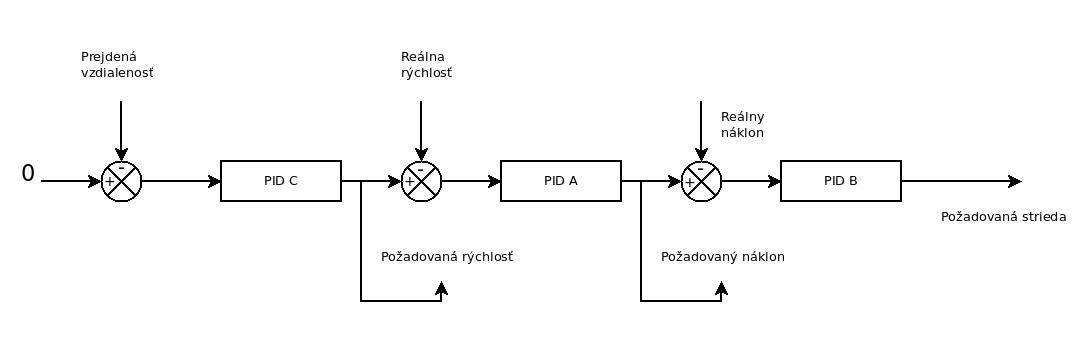
\includegraphics[width=11cm]{additionalPid}
\caption{Upravený RS}
\label{fig:thridPID}
\end{figure}


Ďalšou metódou, ktorá mala pôvodne byť súčasťou hlavnej časti RS robota, bolo meranie elektrického prúdu vstupujúceho do H-mostíka. Myšlienkou bolo navrhnúť a skonštruovať elektrický obvod, ktorý by s použitím tohto merania a dát z mikropočítača bol schopný generovať požadovaný prúd pre motory. 

Výhodou tohto postupu by bolo presnejšie riadenie motorov. Pri nízkych rýchlostiach je totiž točivý moment motorov úmerný prúdu, ktorý nimi tečie - nie napätiu samotnému. Pri balansovaní na mieste kde sú potrebné rýchle a presné reakcie motorov, by sme teda teoreticky mohli priamym riadením momentu motorov dosiahnuť menšie oscilácie pri pohybe.

Meranie prúdu bolo zabezpečené rezistorom s malým odporom \figurename~\ref{fig:currentSensor} zaradeným do série s H-mostíkom. Meraním úbytku napätia na tomto odpore sme pri známom odpore $R$ schopný vypočítať prúd tečúci odporom do H-mostíka. Toto zapojenie bolo realizované na nami navrhnutom shielde a v praxi sme takto boli naozaj schopný zistiť prúd do motorov.

%Tento spôsob riadenia robota ale nebol nakoniec nutný keďže relatívne jednoduchší spôsob generovania PWM signálu priamo mikropočítačom sa javil ako dostatočný. Merania prúdu tak slúžia skôr na účely monitoringu činnosti robota a ich ukážka bude poskytnutá čitateľovi v nasledujúcej kapitole.


 
  

 

\chapter{Laboratórne overenie funkčnosti}

V tejto kapitole predstavíme vlastnosti nami skonštruovaného robota pri laboratórnych testoch. Zameriame sa prevažne na správanie sa robota v režimoch statického balansovania a jeho schopnosť presúvať sa po šikmých plochách.

Pri režime statického balansovania na mieste sa zameriame na priemernú odchýlku od nulového náklonu, amplitúdu oscilácií a celkovú prejdenú vzdialenosť (so zaradením PIDu C aj bez neho).

Všetky grafy požité v tejto kapitole boli vytvorené s použitím nami napísaného python scriptu a dáta v nich zobrazené boli získané prostredníctvom sériovej komunikácie medzi počítačom a robotom.  

\section{Základné parametre robota}
Pre nami vytvoreného robota sme namerali nasledujúce parametre. Tie by mali byť dostatočné pre vytvorenie jednoduchého matematického modelu tohto robota.

\begin{multicols}{2}
\begin{itemize}
\item{$R = 7,2 ~\Omega$}
\item{$K_e = 3,34x10^{-1}$}
\item{$K_m = 9,3x10^{-2}$}
\item{$J_k = 1,598x10^{-3}~ kgm^{2}$}
\item{$J_s = 4,025x10^{-2}~ kgm^{2}$}
\item{$r = 3,4x10^{-2}~ m$}
\item{$m_k = 4,7x10^{-2}~ kg$ss}
\item{$m_p = 1,07 ~kg$}
\item{$L = 0,145 ~m$}
\end{itemize}
\end{multicols}

Pri meraní zotrvačnosti kolesa sme použili vzorec \ref{eq:J_wheel}:
\begin{equation}
J_k = m_kr^2
\label{eq:J_wheel}
\end{equation}

a pre zotrvačnosť celého robota:
\begin{equation}
J_s = \dfrac{m_pgLT^2}{4\pi^2}
\label{eq:J_robot}
\end{equation}
kde $T$ je perióda oscilácie robota okolo osi kolies po vychýlení o malý uhol.


\section{Parametre robota pri balansovaní na mieste}
Pri balansovaní na mieste môže užívateľ zvoliť z dvoch režimov prevádzky. V prvom režime robot balansuje bez toho aby sa snažil udržať počiatočnú pozíciu, v druhom sleduje celkovú prejdenú vzdialenosť a snaží sa ju udržať na minime. Druhý stav je výhodný najmä v prípade ak sa robot nachádza na naklonenej plošine, kde mu sledovanie prejdenej vzdialenosť umožňuje pridávať rýchlosť natoľko aby sa udržal v nehybnosti.

Testovanie správania robota prebiehalo po pripojení k počítaču dlhým, flexibilným káblom, ktorý nám umožnil komunikáciou cez sériovú linku zhromaždiť údaje o stave robota v jednotlivých časových okamihoch. Pomocou týchto dát boli následne vytvorené grafy zobrazené na  \figurename~\ref{fig:combination}. Na osi Y sa nachádzajú odchýlky od pravého uhla pre jednotlivé sledované vzorky. Čas medzi jednotlivými vzorkami bol $t_vz = 50ms$, čiže celkový časový interval, počas ktorého sme sledovali správanie robota trval 50 sekúnd.



\begin{figure}[h]
\centering
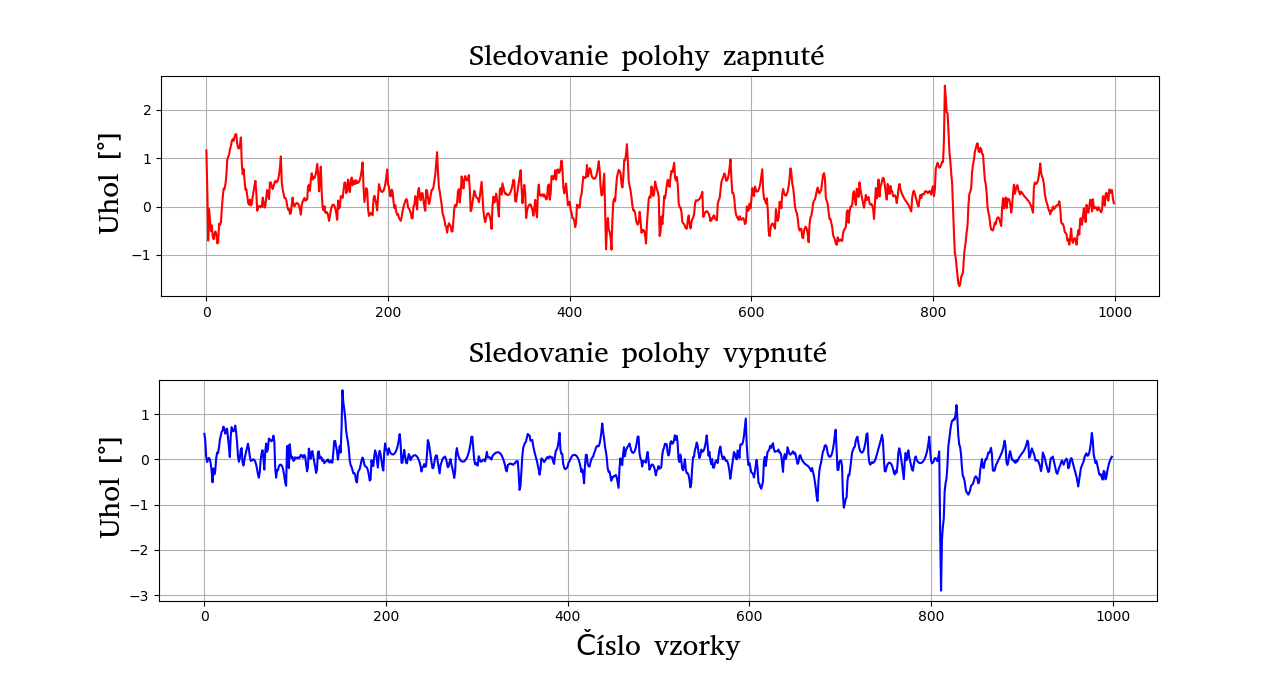
\includegraphics[width=16cm]{combination}
\caption{Náklon robota v čase}
\label{fig:combination}
\end{figure}   

Z porovnania grafov na \figurename~\ref{fig:combination} je zrejmé, že pri vypnutom sledovaní polohy bol robot schopný presnejšie regulovať uhlovú odchýlku od pravého uhla. V tomto režime odchýlka málokedy prekročila hodnotu 1°, čo sa nedá povedať o režime, v ktorom bolo zapnuté sledovanie polohy. Nevýhodou ale bolo, že aj za relatívne krátky čas merania došlo k posunu robota o viac než $5~cm$ oproti počiatočnej polohe, čo v prípade merania v druhom režime nebol problém. Pri sledovaní polohy vzdialenosť robota od počiatočnej polohy nikdy výrazne neprekročila $5~cm$ pričom mal vždy robot tendenciu vracať sa do počiatočnej polohy a oscilovať okolo nej \figurename~\ref{fig:zmena_polohy}.
 
\begin{figure}[h!]
\centering
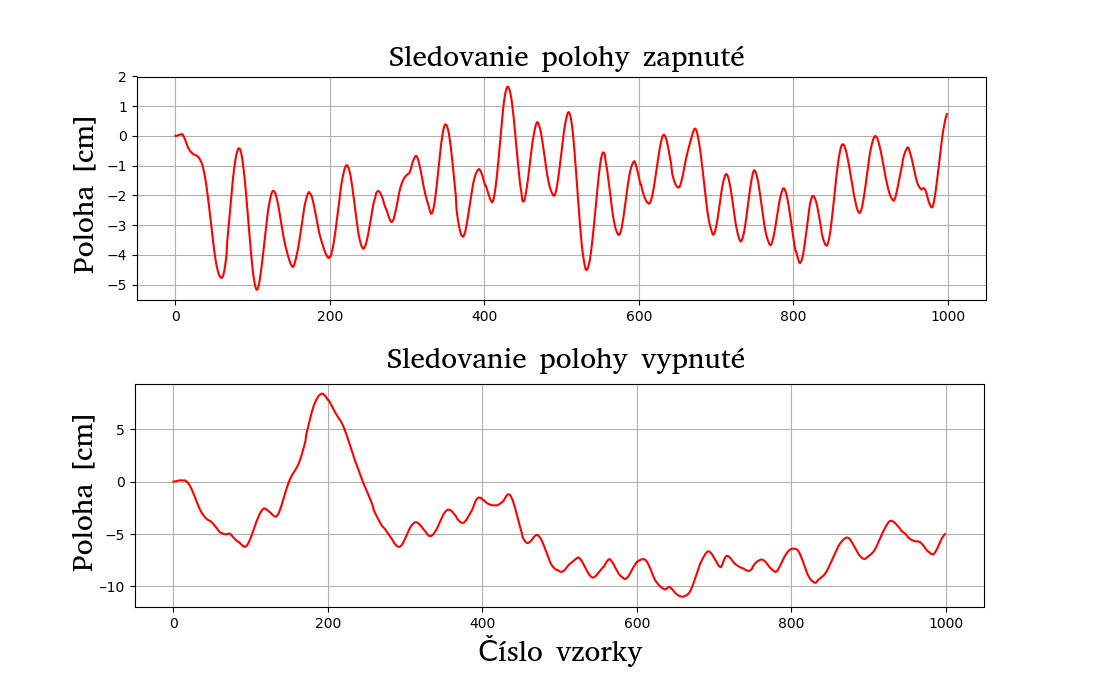
\includegraphics[width=16cm, height=7cm]{zmena_polohy}
\caption{Zmena polohy robota počas testu}
\label{fig:zmena_polohy}
\end{figure}   

Okrem balansovania na rovine sme testovali aj správanie robota pri balansovaní na naklonenej rovine, ktorej sklon bol 15°. Pri tomto teste bol trvalo zapnutý režim so sledovaním polohy keďže, ako už bolo spomenuté, robot nebol bez neho schopný ani zotrvať na plošine. 

Z tohto testu podľa očakávania vyplynulo, že robot vykazoval pri takomto balansovaní zhoršené vlastnosti oproti pohybu na rovine. Oscilácie okolo počiatočného bodu boli väčšie, robot bol však naďalej schopný zotrvať v okolí počiatočnej pozície. Toto ale platilo len pre pohyb v smere náklonu plošiny. Keďže servo pohon nebol v čase písania tejto práce ešte zakomponovaný do riadenia robota, nebol schopný nakloniť šasi tak, aby ostal robot stabilný aj pri pohybe priečnom voči uhlu náklonu plošiny. Tento nedostatok sa prejavoval nerovnomerným pohybom robota, hlavne pri náhlych smeroch jazdy.  


\chapter{Zhrnutie dosiahnutých výsledkov}
V tejto práci sme sa venovali popisu činnosti práce pri návrhu a skonštrovaní dvojolesového balansujúceho robota. Nami vyrobený robot pri meraniach dosiahol uspokojivé výsledy ako pri samostatnom balasovaní na mieste tak aj pri riadenom pohybe na rovine a naklonenej plošine. Za účelom riadenia robota bol taktiež skonštruovaný ovládač, umožňujúci komunikáciu operátora s robotom.  

V rámci práce vznikol taktiež matematický model robota, ktorý nebol priamo použitý v práci, ale v prípade potreby môže byť použitý pri návrhu pokročilejších regulátorov ako napríklad LQR. 




%-------------------------------------------------------
%                     Bibliography
%-------------------------------------------------------

\printbibliography[heading=unchapter,title={Zoznam použitej literatúry}]

%-------------------------------------------------------
%					Čestné vyhlásenie
%-------------------------------------------------------

\makeDeclaration

%-------------------------------------------------------
%						Appendix
%-------------------------------------------------------

\makeAppendixPage
\appendix
\chapter{Ziegler-Nicholsova tabuľka}

\bgroup
\def\arraystretch{1.8}
\begin{table}[h]
\centering
\begin{tabular}{|m{1.7cm}|c|c|c|}
\hline
 & \textbf{$K_p$} & \textbf{$K_i$} & \textbf{$K_d$}\\
\hline
P & $0.5K_p$ & - & - \\
PI & $0.5K_p$ & $\dfrac{0.54K_p}{T_k}$ & - \\
PD & $0.5K_p$ & - & $0.02K_pT_k$ \\
PID & $0.5K_p$ & $\dfrac{1.2K_p}{T_k}$ & $0.075K_pT_k$ \\
\hline
\end{tabular}
\caption{Zieger-Nicholsova tabuľka}
\label{tab:Ziegler-Nichols}
\end{table}
\egroup
% !TeX spellcheck = sk_SK

\chapter{Schéma shieldu}
\begin{figure}[hb]
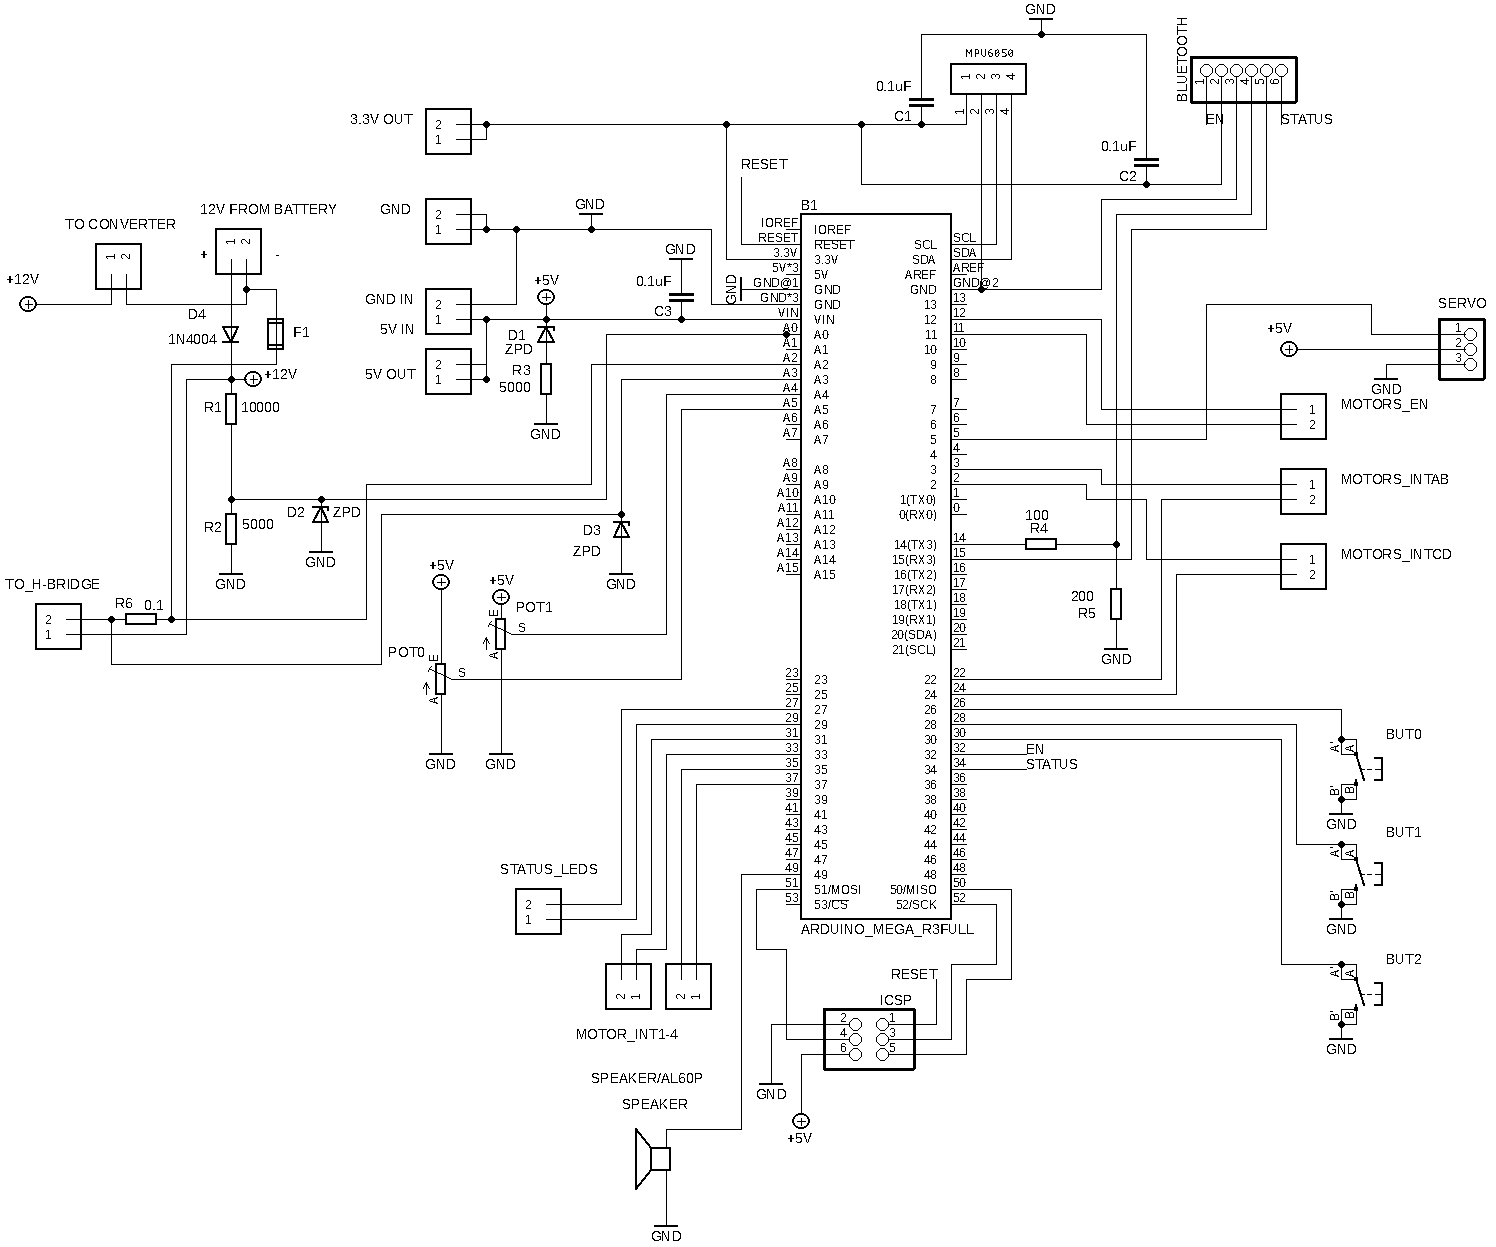
\includegraphics[height=17cm,width=15cm]{schemaShield}
\caption{Schéma shieldu pre Arduino}
\label{fig:schemaShield} 
\end{figure}



\chapter{Schéma H-mostíka}
\begin{figure}[h]
\centering
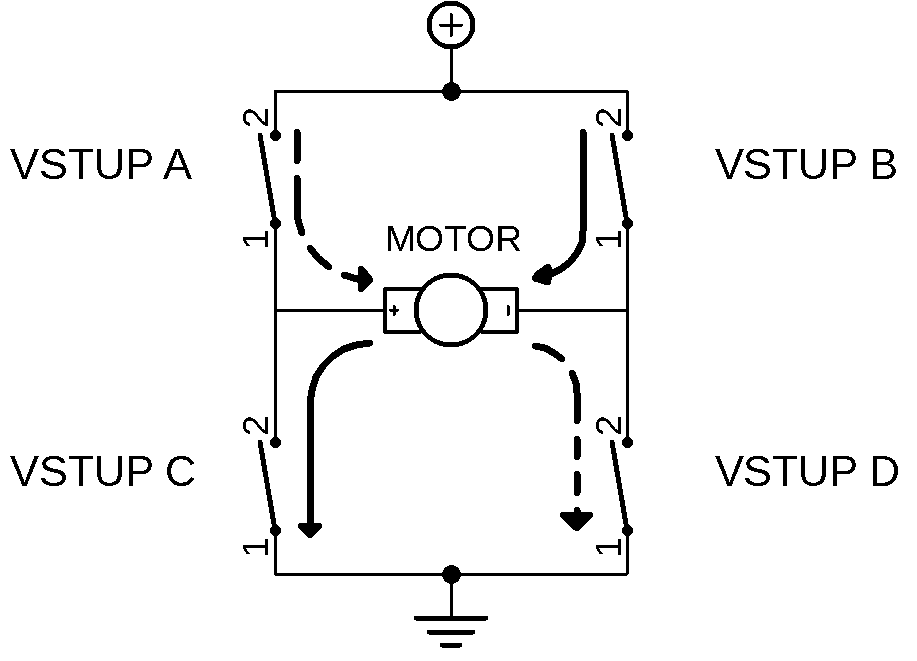
\includegraphics[width=12cm]{h_bridge_scheme}
\caption{Schematické znázornenie H-mostíka}
\label{fig:h_bridge_scheme}
\end{figure}
\chapter{Diagram programu}
\begin{figure}[h]
\centering
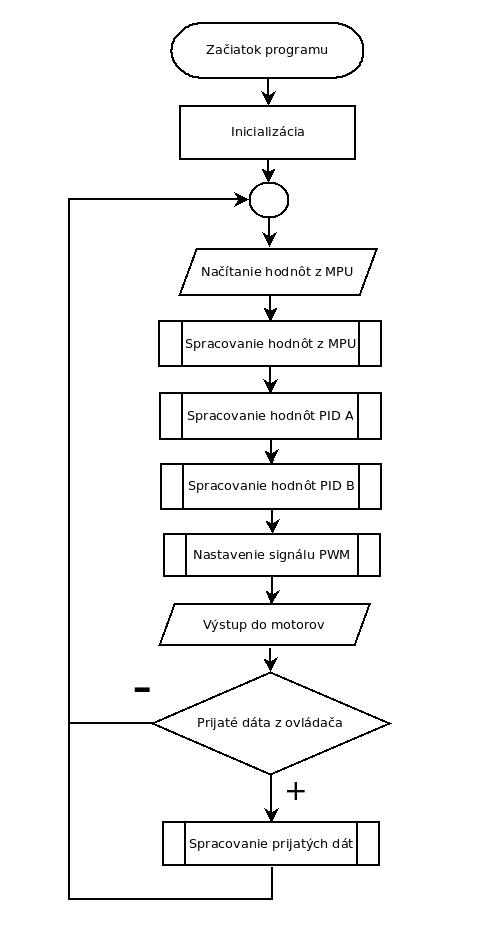
\includegraphics[height=16.5cm]{simple_flowchart}
\caption{Diagram programu.}
\label{fig:simpleFlowchart}
\end{figure}  

\footnotetext{Pozn.: V diagrame nie sú kvôli prehľadnosti znázornené obsluhy prerušení, v ktorých sa aktualizujú údaje z enkodérov.}
\chapter{Výstup z enkodéra}
\begin{figure}[h]
\centering
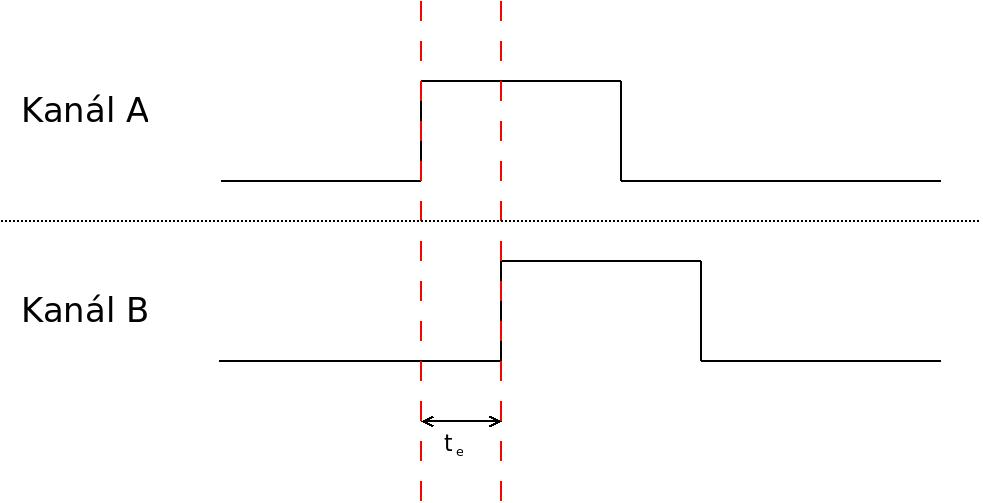
\includegraphics[width = 16cm]{enkoder}
\caption{Výstup z kanálov enkodéra}
\label{fig:enkoder}
\end{figure}
\chapter{Snímanie prúdu}

\begin{figure}[h]
\centering
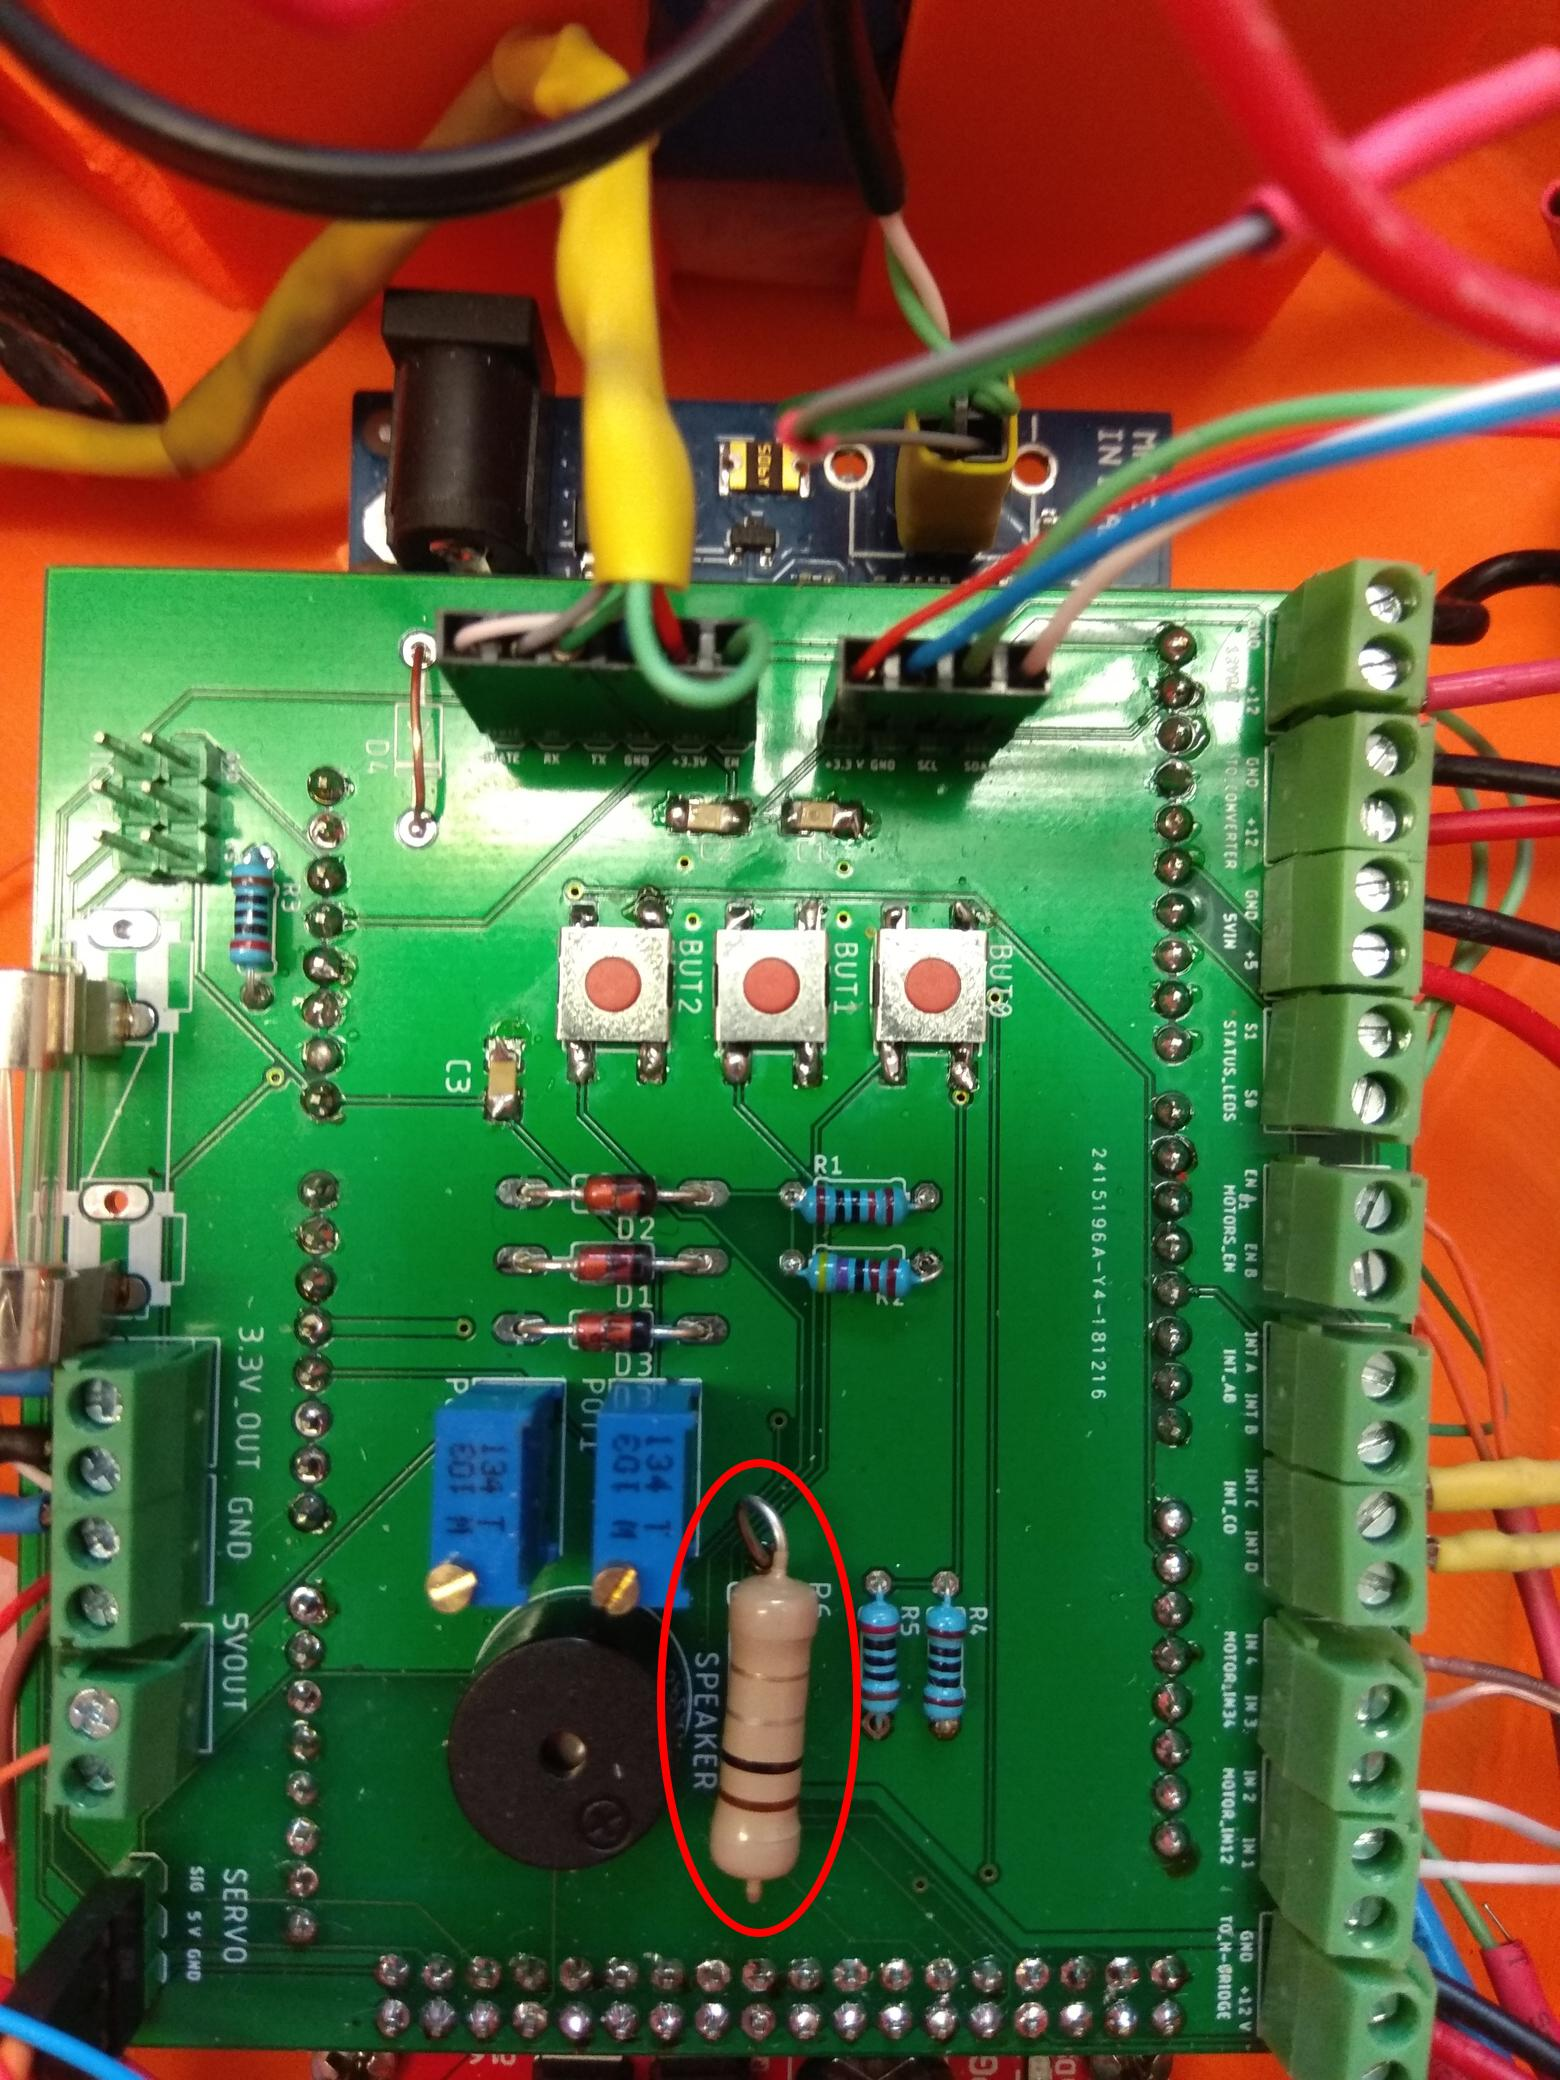
\includegraphics[width=12cm]{shield_marked}
\caption{Shield s vyznačeným rezistorom na snímanie prúdu}
\label{fig:currentSensor}
\end{figure}
\end{document}
